\documentclass{../../Template}
\addbibresource{../../Bibliografia.bib} % si quieres incluir la bibliografía

\RequirePackage{transparent}

\RequirePackage{revsymb}


% Define el campo de subtitle como variable
\newcommand{\subtitle}[1]{\gdef\@subtitle{#1}}

\usetikzlibrary{fadings}

% Macro para hacer el título
\newcommand{\MakeTitle}[4]{%
\begin{titlepage} 

      %-----------------------------
      % --- CASO 0: MODO FOTO ----
      %-----------------------------

      \ifcase #1

      \begin{tikzpicture}[remember picture, overlay,x=\paperwidth, y=-\paperheight]
     
      % Fondo de color (opcional)
      \fill[#2] (current page.south west) rectangle (current page.north east);
      
      \node[opacity=1]  at (0.5,0.1) {\includegraphics[width=1.2\paperwidth]{#4}};

      % Sombra para autores
      \shade [opacity=0.3]
          (0.0, 0.23) rectangle (1.5, 0.35);
      \fill [opacity=0.2]
          (0.0, 0.23) rectangle (1.5, 0.35);

      \node [anchor=south west,align=left] at (0.05,0.32) {\fontsize{22pt}{24pt}\selectfont\bfseries \color{white} \theauthor\par};

      % Sombra para Titulo
      \shade [opacity=0.1,color = #2]
          (0.0, 0.35) rectangle (1.5,1.2);
      \fill [opacity=0.4,color = #2!10]
          (0.0, 0.35) rectangle (1.5,1.2);


      \node[anchor=north west,align=left,text width=0.9\paperwidth] at (0.05,0.38) {
        {\fontsize{60pt}{70pt}\selectfont \bfseries\color{white} \thetitle\par}
        \vspace{1em} \\[1 em]

        {\LARGE\itshape\color{white} \@subtitle\par}
        \vspace{3em}
      };

      % Lineas + Caja lado

      \fill [color=#2!50] (-0.2, 0.45) rectangle (-0.05, 0.36);

      
      \draw [ultra thick, opacity=0.8, color=white] (0.0,-1.5) -- (0.0,1.5);
      \draw [ultra thick, opacity=0.8, color=white] (-1.5,0.35) -- (1.5,0.35);
      
      \end{tikzpicture}

    
      
      %-----------------------------
      % --- CASO 2: MODO SIMPLE ----
      %-----------------------------

      \or 

      \begin{tikzpicture}[remember picture, overlay,x=\paperwidth, y=-\paperheight]
     
      
      % Fondo de color (opcional)
      \fill[#2] (current page.south west) rectangle (current page.north east);

      % Patron de color al fondo: 


      % Fondo (patron)

      % Sombra para autores
      \shade [ opacity=0.3, left color=#3, right color=#2]
          (0.0, 0.0) rectangle (1.5, 0.15);
      \node [anchor=north west,align=left] at (0.05,0.03) {\fontsize{22pt}{24pt}\selectfont\bfseries \color{white} \theauthor\par};

      % Sombra para Titulo
      \shade [opacity=0.4, left color=#3, right color=#2]
          (0.0, 0.15) rectangle (1.5,1.2);
          
      \fill [ opacity=0.3, color = #3]
          (-0.2, 0.15) rectangle (-0.01, 0.3);

      \node[anchor=north west,align=left,text width=0.9\paperwidth] at (0.05,0.18) {
        {\fontsize{56pt}{66pt}\selectfont \bfseries\color{white} \thetitle\par}
        \vspace{1em} \vspace*{2em}

        {\LARGE\itshape\color{white} \@subtitle\par}
        \vspace{3em}
      };
      \end{tikzpicture}
      
      %-----------------------------
      % --- CASO 3:            ----
      %-----------------------------

      \fi
      

    \null % Para evitar espacios verticales no deseados
    \thispagestyle{empty}
    \clearpage
  \end{titlepage}
}

% Para que \title y \author funcionen con \thetitle y \theauthor
\pretitle{\gdef\thetitle}
\preauthor{\gdef\theauthor}




%----------------------------------------------------------------------------
% ÍNDICE PERSONALIZADO
%----------------------------------------------------------------------------

\addto\captionsspanish{\renewcommand{\contentsname}{Índice general}}

\newlength{\fraseancho}
\newcommand{\hLinefill}[1]{\rule[0.5ex]{#1}{0.4pt}}

% Lo que se ejecutará al LEER el .toc
\DeclareRobustCommand{\TOCNewPart}[1]{%
  \par\begingroup
    \parindent=0pt
    \vspace{0.6\baselineskip}%
    \Large\bfseries
    \settowidth{\fraseancho}{#1}%
    \hLinefill{\dimexpr(0.95\linewidth-\fraseancho)/2\relax}%
    \hspace*{4mm}#1\hspace*{4mm}%
    \hLinefill{\dimexpr(0.95\linewidth-\fraseancho)/2\relax}%
    \par\vspace{0.3\baselineskip}%
  \endgroup
}

% Escribimos la llamada al macro anterior dentro del .toc
\newcommand{\NewPart}[1]{%
  \addtocontents{toc}{\protect\TOCNewPart{#1}}%
}

% Macro De Ejemplo

\RequirePackage[most]{tcolorbox}
\tcbuselibrary{skins}

\newcounter{Teorema}[chapter]
\newcounter{Definicion}[chapter]

%%%%%%%%%%%%%%%%%%%%%%%%%%%%%%%%%%%%%%%%%%%%%%%%%%%%%
% Ejercicio

\newcounter{exercise}[chapter]
\renewcommand{\theexercise}{\thechapter.\arabic{exercise}}

% Entorno Ejercicio
\newenvironment{Ejercicio}[1][]{%
  \refstepcounter{exercise}% <-- ancla de hyperref
  \begin{tcolorbox}[
  colback=Gray!40,
  colframe=Gray!40,
  sharp corners,
  boxrule=0pt,
  left=5pt,
  right=5pt,
  top=5pt,
  bottom=5pt,
  top=1.0em,          % margen superior interno (por encima del título y contenido)
  before title={\vspace{0.5em}}, % añade espacio encima del título
  %%
    title={\textcolor{black}{\bfseries \large Ejercicio~\theexercise}}, #1]%
}{%
  \end{tcolorbox}%
}

%%%%%%%%%%%%%%%%%%%%%%%%%%%%%%%%%%%%%%%%%%%%%%%%%%%%%%%
% Ejemplo

\newcounter{example}[chapter]
\renewcommand{\theexample}{\thechapter.\arabic{example}}

% Entorno Ejemplo

\newenvironment{Ejemplo}[1][]{%
  \refstepcounter{example}% <-- ancla de hyperref
  \begin{tcolorbox}[
  enhanced,         %
  colback=Gray!20,  %
  colframe=Gray!20, %
  sharp corners,    %
  left=5pt,         %
  right=5pt,        % 
  top=1.0em,        % margen superior interno (por encima del título y contenido)
  bottom=5pt,       %
  borderline south={3pt}{-3pt}{Gray}, % ← franja a la izquierda
  borderline north={3pt}{-3pt}{Gray}, % ← franja a la izquierda
  before title={\vspace{0.5em}}, % añade espacio encima del título
  title={\textcolor{black}{\bfseries Ejemplo~\theexample}}, #1]%
}{%
  \end{tcolorbox}%
}


%%%%%%%%%%%%%%%%%%%%%%%%%%%%%%%%%%%%%%%%%%%%%%%%%%%
% Teorema


\newcounter{theorem}[chapter]
\renewcommand{\thetheorem}{\thechapter.\arabic{theorem}}

% Entorno Teorema

\newenvironment{Teorema}[1][]{%
  \refstepcounter{theorem}% <-- ancla de hyperref
  \begin{tcolorbox}[
  enhanced,         %
  colback=Gray!30,  %
  colframe=Gray!30, %
  sharp corners,    %
  left=5pt,         %
  right=5pt,        % 
  top=1.0em,        % margen superior interno (por encima del título y contenido)
  bottom=5pt,       %
  borderline west={3pt}{-3pt}{Black!60}, % ← franja a la izquierda
  before title={\vspace{0.5em}}, % añade espacio encima del título
  title={\textcolor{black}{\bfseries Teorema~\thetheorem}}, #1]%
}{%
  \end{tcolorbox}%
}


%%%%%%%%%%%%%%%%%%%%%%%%%%%%%%%%%%%%%%%%%%%%%%%%%%%
% Definicion


\newcounter{definition}[chapter]
\renewcommand{\thedefinition}{\thechapter.\arabic{definition}}

% Entorno definicion

\newenvironment{Definicion}[1][]{%
  \refstepcounter{definition}% <-- ancla de hyperref
  \begin{tcolorbox}[
  enhanced,         %
  colback=Gray!20,  %
  colframe=Gray!20, %
  sharp corners,    %
  left=5pt,         %
  right=5pt,        % 
  top=1.0em,        % margen superior interno (por encima del título y contenido)
  bottom=5pt,       %
  borderline west={3pt}{-3pt}{Black!40}, % ← franja a la izquierda
  before title={\vspace{0.5em}}, % añade espacio encima del título
  title={\textcolor{black}{\bfseries Definición~\thedefinition}}, #1]%
}{%
  \end{tcolorbox}%
}



%%%%%%%%%%%%%%%%%%%%%%%%%%%%%%%%%%%%%%%%%%%%%%%%%%%
% Resalte


\newenvironment{Resalte}[1][]{%
  \begin{tcolorbox}[
  enhanced,         %
  colback=Gray!20,  %
  colframe=Gray!20, %
  sharp corners,    %
  left=5pt,         %
  right=5pt,        % 
  %left skip = 1cm,
  %rigth skip = 1 cm
  top=1.0em,        % margen superior interno (por encima del título y contenido)
  bottom=5pt,       %
  ]
}{%
  \end{tcolorbox}%
}

% Definiciones del título
\title{Interacción \\ Radiación-Materia}
\subtitle{Partículas Cargadas y No Cargadas}
\author{Daniel Vázquez Lago}

% Documento

\begin{document}
\MakeTitle{1}{red!80!black}{Snow1}

\setlength{\parskip}{2.2mm} % Cambia el espacio entre párrafos

\newpage

\tableofcontents

\NewPart{Introducción}
\chapter{Dispersiones}

\section{Teoría de dispersiónes: mecánica clásica y  mecánica cuántica}

\subsection{Mecánica clásica}


\subsection{Mecánica cuántica}

Para describir la dispersión de una partícula por un potencial (Coulomb) en la mecánica cuántica en principio deberíamos estudiar la evolución temporal de un paquete de ondas, que representará la partícula incidente con una energía (y anchura) y una localización espacial (y anchura). Sin embargo, se suelen usar ondas planas, ya que en general las dimensiones del paquete de ondas suele ser mucho más grande que el tamaño del rango efectivo del potencial. La expresión de Rutherford no es una excepción.  

%Para poder entender como se obtiene en la mecánica cuántica la expresión de la sección eficaz lo primero que debemos hacer es entender que la sección eficaz está realcionada directamente con el cuadrado de la amplitud de probabilidad:

%%\begin{equation}
%    \dv{\sigma}{\Omega} = |f(\theta,\varphi)|^2 
%%\end{equation}
%Uno podría plantearse ¿por qué es así? En la mecánica cuántica la sección eficaz diferencial representa la probabilidad de que una partícula salga dispersada en un ángulo sólido diferencial $\D \Omega$, aunque también nos habla de la tasa de partículas que atarviesan una superficie diferencial perpendicular $\D \Omega$. En la mecánica cuántica toda probabilidad es representada por una amplitud de probaiblidad por su complejo, por lo que la relación es directa. 


Partimos de la ecuación de Schrödinger no relativista (masa $m$):
\begin{equation}
i\hbar\,\partial_t\psi=\left(-\frac{\hbar^2}{2m}\nabla^2+V\right)\psi.
\end{equation}
Restando la ecuación conjugada se obtiene la \emph{ecuación de continuidad}
\begin{equation}
\partial_t \abs{\psi}^2 + \nabla\cdot\mathbf{j}=0,
\end{equation}
con \emph{corriente de probabilidad}
\begin{equation}
{\;\mathbf{j}=\frac{\hbar}{m}\,\Im\!\big(\psi^{*}\nabla\psi\big)\;}
\qquad \text{(sustituir $m\to \mu$ si se usa masa reducida).}
\end{equation}

Lejos del blanco ($r\to\infty$), la función de onda toma la forma estándar (no es más que una suposición, una posible solución)
\begin{equation}
\psi(\mathbf r)\;\xrightarrow{r\to\infty}\; e^{ik z}
\;+\; \frac{f(\theta,\phi)}{r}\,e^{ik'r},
\end{equation}
donde $e^{ik z}$ es la onda plana incidente (número de onda $k$) y
$(f/r)\,e^{ik'r}$ es la onda esférica saliente (número de onda $k'$).

Para $\psi_{\rm in}=e^{ikz}$,
\begin{equation}
\mathbf j_{\rm in}=\frac{\hbar}{m}\,\Im\!\big(\psi_{\rm in}^*\nabla\psi_{\rm in}\big)
=\frac{\hbar k}{m}\,\hat{\mathbf z},
\qquad
\Rightarrow\quad
j_{\rm in}=\frac{\hbar k}{m}.
\end{equation}

Para $\psi_{\rm sc}=\dfrac{f(\theta,\phi)}{r}\,e^{ik'r}$, con $f$ independiente de $r$,
\begin{equation}
\partial_r\!\left(\frac{e^{ik'r}}{r}\right)
=\left(\frac{ik'}{r}-\frac{1}{r^2}\right)e^{ik'r}.
\end{equation}
Usando $\mathbf j=(\hbar/m)\Im(\psi^*\nabla\psi)$, el componente radial dominante a gran $r$ es
\begin{equation}
{\;j_r^{(\rm sc)}=\frac{\hbar k'}{m}\,\frac{\abs{f(\theta,\phi)}^2}{r^2}\;}.
\end{equation}
(El término $\propto 1/r^3$ es real y no contribuye a la parte imaginaria.)

El número de partículas por unidad de tiempo que atraviesan el casquete sólido $d\Omega$ a radio $r$ es
\begin{equation}
\frac{dN}{dt}=j_r^{(\rm sc)}\,r^2\,d\Omega
= \frac{\hbar k'}{m}\,\abs{f(\theta,\phi)}^2\, d\Omega.
\end{equation}
Por definición,
\begin{equation}
{\;
\frac{d\sigma}{d\Omega}
=\frac{(dN/dt)}{j_{\rm in}}
=\frac{\hbar k'}{m}\frac{\abs{f}^2}{\hbar k/m}
=\frac{k'}{k}\,\abs{f(\theta,\phi)}^2\;}.
\end{equation}
Aquí aparece el factor cinemático \emph{espacio de fases/flujo} $k'/k$. Se puede relacionar con la energía, con expresiones diferentes en función del a energía inicial de la partícula. 

\begin{itemize}
\item \textbf{No relativista.} Como $k\propto \sqrt{E_{\rm k}}$,
\begin{equation}
\frac{k'}{k}=\sqrt{\frac{E'_{\rm k}}{E_{\rm k}}}.
\end{equation}

\item \textbf{Relativista } Para $E\gg mc^2$, $p\approx E/c$ y $k\propto p$,
\begin{equation}
\frac{k'}{k}\approx \frac{E'}{E}.
\end{equation}
\end{itemize} 
El factor $k'/k$ ya surge al trabajar \emph{en un mismo sistema de referencia} (p.\,ej.\ LAB) a partir de la razón
\emph{corriente saliente} / \emph{flujo incidente}. Si además se pasa del CM al LAB, aparece un \emph{Jacobiano angular} $d\Omega_{\rm cm}/d\Omega_{\rm lab}$, pero es un factor \emph{distinto} del $k'/k$.

\section{Análisis en ondas parciales}

\subsection{Introducción}

\subsection{Fases}

\subsection{Teorema óptico}

\section{Aproximación de Born}

\subsection{Primera aproximación de Born}

\subsection{Teoría de Born}

\section*{Ejercicios}
\addcontentsline{toc}{section}{Ejercicios}


\begin{Ejercicio}{Sección eficaz de Rutherford con modelo atómico de Fermi} \label{Ej:01.01}
    Obten la expresión de la sección de eficaz de Rutherford, usando la aproximación de Born con ondas planas incidentes y salientes con el potencial de Coulomb:

    \begin{equation}
        V(r) = \frac{zZe^2}{4\pi \varepsilon} \frac{1}{r}
    \end{equation}
\end{Ejercicio}




\NewPart{Interacción radiación materia}

\chapter{Partículas Cargadas}

\section{Dispersión de Rutherford}

\subsection{Introducción}

Rutherford describió la dispersión de una partícula $\alpha$ por núcleos atómicos (con $m_\alpha \ll M, z=2$) sobre una trayectoria hiperbólica a través del potencial de Coulomb. La energía total viene dada como la suma de la energía cinética y potencial, y permanece \textit{constante} sobre toda la trayectoria:

\begin{equation}
    E(r) = E_K(r) + E_p (r) \qquad  E_p (r) = \frac{ z Z e^2}{4\pi \varepsilon_0} \frac{1}{R} \qquad E_K (r) = \frac{1}{2} m_\alpha v_\alpha^2
\end{equation}
La distancia de máxima aproximación se define como la distancia a la cual se para una partícula con parámetro de impacto $b=0$, i.e. colisión frontal. Así, denotando $E_K$ como la \textit{energía cinética inicial}, tenemos que

\begin{equation}
   E_K = \frac{zZe^2}{4\pi\varepsilon_0} \frac{1}{D_{\alpha-N}}
\end{equation}
aunque lógicamente esta expresión no será del todo cierta, ya que el potencial no es infinito en $r=0$, debido a que el núcleo es finito. Aún así es una buena aproximación.


\subsection{Relación entre el parámetro de impacto y el ángulo de dispersión}

El momento transferido en la interacción, siempre y cuando $|\pn_i |= |\pn_f|=p$ vale 

\begin{equation}
    \Delta p = 2 p \sin (\theta/2)
\end{equation}
siendo $\theta$ el \textbf{ángulo de dispersión}. Es fácil de deducir matemáticamente, pero incluso físicamente tiene sentido: cuando $\theta=\pi$ la trasferencia de momento es máxima (la partícula se da la vuelta completamente) lo que implicla un intercambio de $2$ veces el momento inicial. Definimos como \textbf{parámetro de impacto} 

\begin{equation}
    b = r \sin \theta
\end{equation}
cuando la partícula está en el infinito. Además, también se conserva el momento angular $L = |\rn \times \pn|=L p \sin \theta$, lo que lleva a la relación 

\begin{equation}
    v_i b = \omega r^2
\end{equation}
siendo $\omega=\dv{\phi}{t}$ en el vértice, definiendo $\phi$ como el ángulo entre el vértice y la partícula desde el núcleo. En el vértice, que es el punto en el cual la posición respecto el átomo y el momento lineal de la partícula son perpendiculares. Tenemos que en el infinito

\begin{equation}
    L_\infty = |\rn \times \pn | = m_\alpha b v_i        
\end{equation}
mientras que en el vértice: 

\begin{equation}
    L_a = |\rn \times \pn | = r p \sin 90^\circ = r m_\alpha \left( r \dv{\phi}{t} \right)  = m_\alpha \omega r^2
\end{equation}  
El momento transferido $\Delta p$ se calcula como la acción total en el tiempo de la fuerza de Coulomb proyectada sobre el eje de la hipérbola, tal que

\begin{equation}
    \Delta p = \int_{-\infty}^{\infty} F_{\Delta p} \D t  = A \int_{-\frac{\pi-\theta}{2}}^{\frac{\pi-\theta}{2}} \frac{\cos \phi}{r^2} \pqty{\dv{t}{\phi} \D \phi}  = \frac{A}{b v_i} \int_{-\frac{\pi-\theta}{2}}^{\frac{\pi-\theta}{2}} \cos \phi \D \phi = \frac{2 A}{v_i b} \cos (\theta/2) \quad A = \frac{zZe^2}{4\pi \varepsilon_0}
\end{equation}
de lo que se puede deducir que el parámetro de impacto $b$ y el ángulo de dispersión se relacionan tal que:

\begin{equation}
    b = \frac{1}{2} D_{\alpha - N} \cot (\theta/2) = \frac{1}{2} D_{\alpha-N} \sqrt{\frac{1+\cos \theta}{1-\cos \theta}} \qquad D_{\alpha-N} = \frac{zZe^2}{4\pi \varepsilon_0} \frac{1}{E_K}
\end{equation}
siendo $\D_{\alpha-N}$ la distancia de máxima aproximación y $E_K$ la energía cinética. 

\subsection{La sección eficaz diferencial de Rutherford}

La dispersión de las partículas alfa que halló Rutherford la describió en función de su sección diferencial, tal que:

\begin{Resalte}
\begin{equation}
    \dv{\sigma_{\Ruth}}{\Omega} =  \pqty{\frac{D_{\alpha-N}}{4}}^2 \frac{1}{\sin^4 \frac{\theta}{2}} \qquad D_{\alpha-N} = \frac{zZe^2}{4\pi\varepsilon_0} \frac{1}{E_K}
\end{equation}
\end{Resalte}
Esta ecuación, aunque fue calculado con la mecánica clásica, también puede ser hallada en la mecánica cuántica, usando las aproximaciones de Born a primer orden ya vistas. 
 
Como podemos comprobar, \textit{diverge} para $\theta=0$, lo cual es debido al carácter ideal del núcleo puntual. La razón por la que en realidad no diverge, o la solución a esta divergencia, es que la carga nuclear está apantallada por los \textit{electrones orbitales atómicos}, lo que conduce a un ángulo mínimo $\theta_{\min}$. La dispersión hacia atrás ($\theta \to \pi, b \to 0$) tampoco se logra nunca, debido al radio finito del núcleo. 

En ambos casos el punto es el mismo: debido a la localización de la partícula al interaccionar con el potencial, el propio principio de incertidumbre genera un $\Delta p$ relacionado directamente con el rango efectivo del potencial $x$, tal que

\begin{equation}
\Delta p \approx \frac{\hbar}{x}
\end{equation}
y, debido a esto y la geometría, el ángulo medio 
\begin{equation}
    \bar{\theta} = \frac{\Delta p}{p} 
\end{equation}
que se puede ver geométricamente. De todos modos tampoco hace falta entenderlo físicamente, basta con ver que las correciones físicamente correctas al potencial de Coulomb (al no ser, los átomos, ``objetos cargados'', ni los núcleos ``cargas puntuales'') basta para ver que aparecen un ángulo mínimo y máximo.

\subsection{Ángulo mínimo: corrección por apantallamiento}
Un modelo que tiene en cuenta el apantallamiento es el \textit{modelo atómico estadístico de Fermi}, el cual introduce una exponencial tabulada por un \textit{radio efectivo} $\alpha_{TF}$ de tal modo que el potencial de Coulomb no caiga ``lentamente''. Así pues: 

\begin{equation}
    V_{TF} (r) = \frac{zZe^2}{4\pi\varepsilon_0} \frac{1}{r} e^{-\frac{r}{a_{TF}}}
\end{equation}
el \textit{radio efectivo} $a_{TF}$ de la nube electrónica (de Thomas-Fermi) decrece por debajo del radio de Bohr $\alpha_0$ al aumentar $Z$, como $a_{TF}=\frac{\zeta a_0}{\sqrt[3]{Z}}$, debido a la disminución del tamaño de los orbitales más internos, por el teorema de Gauss. 

La aproximación de Born requiere ahora, con $\Delta k = K=(2p/\hbar) \sin(\theta/2) (p=p_i)$ el momento de onda transferido ($p = \hbar k$), el cálculo de la transformada seno de $V_{TF}(r)$, que es finita. Rutherford reciba entonces un \textit{factor corrector} tal que:

\begin{equation}
    \dv{\sigma_{\Ruth}}{\Omega} = \vqty{\frac{2m_\alpha}{\hbar^2}\int_{0}^{\infty} r^2 V_{TF}(r) \frac{\sin Kr}{Kr} \D r }^2 = \pqty{\frac{D_{\alpha-N}}{4}}^2 \frac{1}{\sin^4 \theta/2} \pqty{\frac{1}{1+\frac{1}{K^2 a_{TF}^2}}}
\end{equation}
Cuando $\theta\ll 1$, tenemos que: 

\begin{equation}
    \dv{\sigma_{\Ruth}}{\Omega} = \frac{D_{\alpha-N}^2}{\theta^4} \frac{1}{\bqty{1+\pqty{\frac{\theta_{\min}^2}{\theta^2}}^2}} = \frac{D_{\alpha-N}^2}{\theta^2+\theta_{\min}^2} 
\end{equation}
donde se introduce el concepto el concepto de ángulo mínimo, que como podemos ver viene expresado: 

\begin{equation}
    \theta_{\min} = \frac{\hbar}{p a_{TF}} = \frac{\hbar \sqrt[3]{Z}}{pa_{TF}} = \frac{\hbar c \sqrt[3]{Z}}{a_0 \sqrt{E_K(E_K+2Mc^2)}}  \label{Ec:02-thetamin}
\end{equation}
donde hemos usado que 

\begin{equation*}
    p^2 c^2 = E^2 - m^2 c^4 \Rightarrow p  = \frac{1}{c} \sqrt{E^2 - m^2 c^4 - M^2 c^4} = \frac{1}{c} \sqrt{(E_K + m c^2 + M c^2)^2 - m^2 c^4  - M^2 c^4} 
\end{equation*}
que despreciando la masa de la partícula incidente $m$ frente a $M$
\begin{equation}
    p  \approx \frac{1}{c} \sqrt{E_K (E_K + 2 Mc^2) } 
\end{equation}
La mejora de la aparición de este ángulo mńimo es que ahora \textit{la sección eficaz total es finita}, lo cual se corresponde a un resultado mucho más físico. Este ángulo mínimo tiene un \textit{origen cuántico} debido al \textit{principio de incertidumbre}. Se produce por la localización de la partícula sobre el radio $a_{TF}$, que le imprime un momento \textit{transversal} inevitable $\Delta p$, relacionado con la longitud de onda: 
\begin{equation}
    \theta_{\min} = \frac{\Delta p}{p} \approx \frac{\hbar}{pa_{TF}} = \frac{\lambdabar}{a_{TF}}
\end{equation}
\subsection{Ángulo máximo: corrección por radio finito del núcleo}

El potencial que ve una carga elemental $z$ cerca del núcleo $V(r)$ tiene un plateu en su interior hasta $r=R$ y para $r>R$ adopta la forma de Coulomb $E_p(r)$. Una forma de representar  este potencial es con la ecuación 

\begin{equation}
    V_{FSN} (r) = \frac{zZe^2}{4 \pi \varepsilon_0} \frac{1}{r} \pqty{1-e^{-\frac{2r}{R}}}
\end{equation}
en la \cref{Fig:02.01} vemos la representación de esta función. 

\begin{figure}[H] \centering
    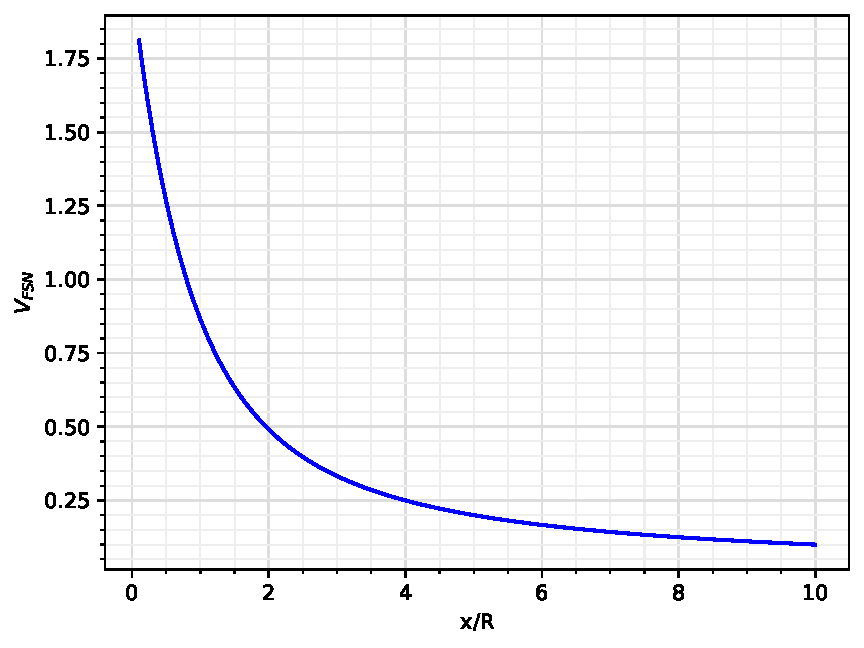
\includegraphics[width=0.6\linewidth]{Images/Ch_02/02-Vfsn.pdf}
    \caption{Representación del potencial $V_{FSN}(r)$. Como podemos comprobar no representa un ``plateu'', pero tampoco hace infinito al potencial en el centro, lo que nos basta.}
    \label{Fig:02.01}
\end{figure}

La nueva expresión de la sección eficaz de Rutherfrod con este potencial vendrá dada por:

\begin{equation}
    \dv{\sigma_{\Ruth}}{\Omega} = \pqty{\frac{D_{\alpha-N}}{4}}^2 \frac{1}{\sin^4(\theta/2)} \frac{1}{\bqty{1+\pqty{\frac{\sin (\theta/2)}{\bar{\theta_{\max}}}}^2}^2}
\end{equation}
Siendo $\bar{\theta_{\max}}$ un parámetro de origen cuántico que suprime la probabilidad de dispersión hacia atrás, siendo solo significativa para $0<\theta<\theta_{\max}<\pi$. Toma el valor:

\begin{equation}
    \bar{\theta}_{\max} = \frac{\hbar}{p R} = \frac{\hbar }{R_0 \sqrt[3]{A} \sqrt{E_K (E_K+Mc^2)}}   \label{Ec:02-tehtamax}
\end{equation}
Ilustra las fluctuaciones transversales que impiden la localización de la hipérbola clásica hacia atrás. 


\section{Dispersión de Mott} 

La dispersión de Mott tiene básicamente 3 correcciones: la correción relativista, es decir, la correción que se hace a la energía y momento cuando partícula tiene una energía cinética inicial de entorno la masa de la partícula; la correción por el espín (para partículas muy relativistas) y la corrección por el retroceso del núcleo (que se da cuando la partícula no tiene una gran masa respecto la de la partícula incidnete). En el marco de la física médica estas tres son suficientes. 

\subsection{Correcciones relativistas}

La correción relativista (aunque no ultrarrelativista) implica el simple intercambio de  $2E_K = p v = m \gamma \beta^2  c^2$, es decir, multiplicar por $\gamma$: 

\begin{equation}
    D_{n-N}  = \pqty{\frac{zZe^2}{4\pi\varepsilon_0}} \frac{1}{\frac{1}{2}m_n \gamma c^2 \beta^2}
\end{equation}
Aunque ahora $D_{n-N}$ no se llama distancia de máxima aproximación, sino \textit{distancia característica efectiva.}


\subsection{Correcciones por espín}

La correción por el espín está relacionada con la \textit{helicidad} $h$, que se define como la proyección del momento sobre el espín: 

\begin{equation*}
    h = \frac{\sn \cdot \pn}{|\sn||\pn|}
\end{equation*}
Este se conserva edebido a la forma de los espinores en el sistema centro de masas cuando tenemos partículas ultrarrelativistas. Un intercambio de dirección del momento sin modificar también la dirección del espín implicaría que se violaría paridad, lo que no puede ocurrir. Esto es lo que expresa el factor: 

\begin{equation}
    f_{\text{espin}} = 1 - \beta^2 \sin^2 (\theta/2) \to \frac{1}{2} \pqty{1+\cos \theta}
\end{equation}
tal que: 

\begin{equation}
    \dv{\sigma_{\text{Mott}}}{\Omega} =  \dv{\sigma_{\Ruth}}{\Omega}  f_{\text{espin}}
\end{equation}
aunque aún queda una corrección. 



\subsection{Correcciones por retroceso del núcleo}

La correción por retroceso del núcleo está relacionada con la asunción de que el núcleo tiene una masa infinita, por lo que no adquire momento y la colisión es totalmente elástica. Sin embargo, si hay un momento transferido $\Delta p$ le imprime cierta energía cinética al núcleo: $\Delta E = {\frac{\pqty{\Delta p}^2}{2M}} = E_K'-E_K$, tal que $p_f\neq p_i$. Como hemos visto, ahora tenemos que tener en cuenta el factor $p'/p$ en la expresión de la sección eficaz, debido al cambio en el espacio de fases, tal que

\begin{equation}
    \dv{\sigma_{\text{Mott}}}{\Omega} = f_{\text{espin}}f_{\text{retroceso}} \dv{\sigma_{\Ruth}}{\Omega}  
\end{equation}
siendo 

\begin{equation}
    f_{\text{retroceso}} = \frac{p'}{p} 
\end{equation}
que en el caso relativista: 

\begin{equation}
    f_{\text{retroceso}} = \frac{p'}{p}  \approx  \frac{E_K'}{E_K}    
\end{equation}
Veamos como se llegan a ellas: 

\begin{equation}
    E_K' = E_K - \Delta E \quad E_K^2 = p^2 c^2 + m_e^2 c^4 \quad \Delta E = {\frac{\pqty{\Delta p}^2}{2M}} \approx \frac{1}{2M} 4 p^2 \sin^2 (\theta/2) = \frac{E_K^2-m_e^2c^4}{2Mc^2} 2 \sin^2 (\theta/2)
\end{equation}
donde hemos usado que $\Delta p^2 = 4 p^2 \sin^2 (\theta/2)$. Esto nos lleva a que:

\begin{equation*}
    \Delta E \approx \frac{E_K^2}{Mc^2} \sin^2 (\theta /2) \Longrightarrow
\end{equation*}
\begin{equation} E_K ' = E_K  \pqty{1 - \frac{E_K}{Mc^2} 2 \sin^2 (\theta/2)} = E_K \pqty{1 - \frac{E_K}{Mc^2} (1  - \cos^2 (\theta) )} \approx \frac{1}{1+\pqty{\frac{E_K}{Mc^2} (1  - \cos^2 (\theta) )}}
\end{equation}
y, consecuentemente, a que el factor de correción por retroceso sea

\begin{equation}
    f_{\text{retroceso}}  = \frac{1}{1+\pqty{\frac{E_K}{Mc^2} (1  - \cos^2 (\theta) )}}
\end{equation}


\subsection{Correcciones por factor de forma nuclear}

El factor de forma nuclear se relaciona con la densidad de carga (distribución de carga) dentro del núcleo, tal que $f(k)$ es :

\begin{equation}
    f(k) = \int_{\text{nucleo}} \rho (\rn) e^{-i \kn \cdot \rn} \D^3 \rn
\end{equation}
tal que la sección eficaz experimental real: 

\begin{equation}
     \dv{\sigma_{\text{exp}}}{\Omega} =  |f_{k}|^2 \dv{\sigma_{\text{Mott}}}{\Omega}
\end{equation}

\section{Dispersiones individuales}
 
La mayor parte e las interacciones de las partículas y la materia se producen como colisiones elásticas de Coulomb con los átomos. Las colisiones o bien pueden ser con los electrones orbitales de los átomos o con el núcleo. En cualquiera de los casos, la trayectoria de las partículas es una hipérbola, aunque en función del signo relativo tendremos que el foco será interior (atractivo) o exterior (repulsivo).

La sección eficaz individual puede escribirse, cuando el ángulo es muy pequeño $(\theta \ll 1)$, cómo: 

\begin{equation}
    \dv{\sigma}{\Omega} = \frac{D_{ab}^2}{\pqty{\theta^2 + \theta_{\min}^2}^2}
\end{equation}
Este ángulo mínimo ya sabemos de donde procede: del apantallamiento de Coulomb de los electrones en los orbitales, y cómo se puede calcular también lo sabemos, dependiendo únicamente de la energía inicial de la partícula, de la carga de la partícula incidente, y de la carga y masa del blanco. En función de $a$ y $b$, esto es, del blanco y partícula incidente, también dependerá  la expresión de $D_{ab}$, tal y como veremos en el siguiente apartado.

\subsection{Clasificación de las colisiones elásticas con la materia}

Aquí podemos ver que principalmente en función de la masa de la partícula (y por ende, de si es relativista o no) tendremos una expresión u otra de la distancia de máxima aproximación/distancia 

\begin{itemize}
    \item Por ejemplo un ion pesado o protón frente a un núcleo. En este caso no suele ser relativista, por lo que la expresión correcta sería
    \begin{equation}
            D_{\alpha-N} = \frac{zZe^2}{4\pi \varepsilon_0} \frac{2}{p_\alpha v_\alpha }
    \end{equation}
    aunque si llegara a ser relativista $p_{\alpha} = m_{\alpha} \gamma_{\alpha} \beta_{\alpha} \beta_{\alpha} c$. 
    \item Cuando hacemos la colisión electrón-núcleo podemos suponer que es siempre relativista (y $z=1$)
    \begin{equation}
            D_{e-N} = \frac{Ze^2}{4\pi \varepsilon_0} \frac{2}{ m_{e} \gamma_{e} \beta_{e}^2 c^2 }
    \end{equation}
    \item Cuando hacemos electrón-electrón orbital: 
    \begin{equation}
            D_{e-e} = \frac{e^2}{4\pi \varepsilon_0} \frac{2}{p_\alpha v_\alpha }
    \end{equation}
    \item Finalmente, cuando hacemos electrón-átomo: 
    \begin{equation}
            D_{e-a} = \sqrt{D_{e-N}^2+ZD_{e-e}^2} = \frac{\sqrt{Z(Z+1)}e^2}{4\pi \varepsilon_0} \frac{2}{\gamma_e m_e \beta^2_e c^2 }
    \end{equation}
\end{itemize}

\subsection{Ángulos de dispersión mínimo y máximo}

Ya hemos revelado como se originan tanto el ángulo mínimo como el ángulo máximo (desviación de la ley de Coulonmb de su carácter puntual), y se corresponden con parámetro de impacto $b \to \infty$ y $b \to 0$ (al final cuando va hacia atrás $b=0$, dispersión frontal, y vicerversa). Recordando la \cref{Ec:02-thetamin} y \cref{Ec:02-tehtamax}, queda claro que el cociente entre $\bar{\theta}_{\max}$ y $\theta_{\min}$, tal que: 

\begin{equation}
    \frac{\bar{\theta}_{\max}}{\theta_{\min}} = \frac{a_F}{R_0 \sqrt[3]{A}} = \frac{a_0}{R_0} \frac{1}{\sqrt[3]{AZ}}  =  \frac{0.423 \times 10^5}{(AZ)^{1/3}} \label{Ec:02-CocienteDeAngulos}
\end{equation}
siendo $a_F$ el radio efectivo del átomo, $a_0$ el radio de Bohr,  y $R_0 \approx 1.2$ fm, que es el tamaño del núcleo de hidrógeno. El comportamiento respecto la energía tanto de $\bar{\theta}_{\max}$ y $\theta_{\min}$ es parecido, ya que ambos dependen del mismo parámetro $p_i$ en el denominador.
Cuando $\bar{\theta_{\max}}>\pi$, se asume que $\theta_{\max} = \pi$, esto es: 

\begin{equation}
    \theta_{\max} = \max \Bqty{\bar{\theta}_{\max}, \pi}
\end{equation}

\subsection{Ángulo cuadrático promedio}

La sección eficaz total es un parámetro muy importante, ya que nos permite hallar cuantas interacciones entre las partículas de un haz incidente y las del blanco material ocurren. Veamos que, si $\theta \ll 1$: 

\begin{equation*}
    \sigma = \int \dv{\sigma}{\Omega} \D \Omega = 2 \pi D \int_0^{\bar{\theta}_{\max}} \frac{\theta   \D \theta}{\pqty{\theta^2 + \theta_{\min}^2}^2} =  2 \pi D \bqty{-\frac{1}{2} \frac{1}{\theta^2 + \theta_{\min}^2}}_{0}^{\theta_{\max}}
\end{equation*}
de lo que se deduce 
\begin{equation}
    \sigma =\pi D^2 \frac{1}{\theta^2_{\min}} \bqty{1-\frac{1}{1+(\theta_{\max}/\theta_{\min})^2}} \approx \frac{\pi D^2}{\theta_{\min}^2}
\end{equation}
(donde hemos usado $\cos \theta \approx \theta$). Ahora, lo sguiente es calcular el \textbf{ángulo cuadrático promedio}, ya que es una medida que nos permite hallar luego el ángulo cuadrático medio para dispersiones múltiples. 

\begin{equation}
    \bar{\theta}^2 = \frac{\int_{0}^{\theta_{\max}} \theta^2  \dv{\sigma}{\Omega} \D \Omega}{\int_{0}^{\theta_{\max}} \dv{\sigma}{\Omega} \D \Omega} = \frac{2\pi D^2}{\sigma} \int_{0}^{\theta_{\max}} \frac{\theta^3 \D \theta}{(\theta^2 + \theta_{\min}^2)^2}
\end{equation}
pudiendo obtener:

\begin{equation}
    \bar{\theta}^2 = \theta_{\min}^2 \bqty{\ln \pqty{1+\frac{\theta^2_{\max}}{\theta^2_{\min}}} - \frac{1}{1+(\theta_{\max}/\theta_{\omega})^2}}  
\end{equation}
dado que $ \frac{\bar{\theta}_{\max}}{\theta_{\min}} \propto a_0 /R_0 \gg 1$, podemos asumir la aproximación: 

\begin{equation}
    \bar{\theta}^2 = \theta_{\min}^2 \ln \pqty{\frac{\theta_{\max}^2}{\theta_{\min}^2}}    \label{Ec:02-AnguloCuadraticoPromedio}
\end{equation}
Si sustituimos $A=2Z$ (y suponemos que $\theta \ll 1, \theta_{\min} \ll \theta_{\max}$ y que $\sigma = \pi D^2 / \theta_{\min}^2$), entonces: 

\begin{equation}
    \bar{\theta}^2 \approx  4 \theta_{\min}^2 \ln \bqty{183 Z^{-1/3}}  \label{Ec:02-AnguloCuadraticoPromedio2}
\end{equation}

\section{Dispersiones múltiples}

Las dispersiones múltiples, a diferencia de las dispersiones individuales, están gobernadas (o mejor dicho, están parametrizadas) en función de: la longitud de radiación $X_0$, el ángulo cuadrático promedio múltiple $\overline{\Theta^2}$, y el poder de dispersión angular másico $T/\rho$. 

\subsection{Ángulo Cuadrático Medio}

Cuando un haz paralelo de partículas incide una lámina, siempre y cuando todos los ángulso de deflexión sean pequeños, podemos obtener un ángulo de desviación cuadrático promedio $\overline{\Theta^2}$. El teorema del límite central (que básicamente habla de como la suma de variables aleatorias procedentes de una misma distribución nos lleva a una gaussiana) nos asegura que 

\begin{equation}
    \overline{\Theta^2} = n \bar{\theta}^2 
\end{equation} 
siendo $n$ el número de colisiones de la partícula (para que esto se cumpla $n>20$).  Vamos a obtener entonces cual es el número de colisiones (promedio) en el absorbente de grosor $t$. Si $\sigma$ es la sección eficaz total

\begin{equation}
    n = \frac{N_a}{V} \sigma t = \rho \frac{N_A}{A} \sigma t \approx \pi \rho \frac{N_A}{A} \frac{D^2}{\theta^2_{\min}} t 
\end{equation}
que si lo juntamos con la \cref{Ec:02-AnguloCuadraticoPromedio} tenemos entonces:

\begin{equation}
    \overline{\Theta^2} = \pi \rho \frac{N_A}{A} D^2 t \ln \pqty{\frac{\theta_{\max}^2}{\theta_{\min}^2}} 
\end{equation}
ahora podemos aplicar la ecuación \cref{Ec:02-CocienteDeAngulos} para poder reexpresar $\overline{\Theta^2}$ en función de $Z$ y $A$, tal que así 

\begin{equation}
    \overline{\Theta^2} = \pi \rho \frac{N_A}{A} D^2 t \bqty{2 \ln \pqty{\frac{a_0}{R_0} \frac{1}{\sqrt[3]{AZ}}}}. 
\end{equation}
que, en función de la partícula incidente y del blanco, siempre podremos aproximar (bien podemos suponer $A \approx 2 Z$, un valor para $a_0$ y $R_0$...). La aproximación usando esto último es (\cref{Ec:02-AnguloCuadraticoPromedio2}) obtenida es: 

\begin{equation}
    \overline{\Theta^2} = 4 \pi \rho D^2 t \frac{N_A}{A} \ln \pqty{183 Z^{-1/3}}
\end{equation}


\subsection{Poder de dispersión angular másico}

La siguiente definción de interés es el \textbf{poder de dispersión angular másico}, qeu se define como

\begin{equation}
    \frac{T}{\rho} = \frac{\overline{\Theta^2}}{\rho t}
\end{equation}
con unidades $[\unit{rad^2 cm^2 /g}]$ ($T [\unit{rad^2 cm^{-1}}]$). 


\subsection{Longitud de radiación}

La longitud de radiación $X_0$ se define como 

\begin{equation}
    \frac{1}{X_0} = 4 \alpha \frac{N_A}{A} Z (Z +1) r_e^2 \ln \pqty{\frac{183}{Z^{1/3}}}
\end{equation}
que es la expresión que surge de \cref{Ec:02-AnguloCuadraticoPromedio2} entre otras. Esta variable representa la distancia promedio que una partícula cargada relativista viaja en el medio para que su enerǵia se reduzca un factor $1/e$ (al 36.8 \%) respecto su valor inicial. También representa 7/8 del camino libre medio necesario para que se emita un par $e^+e^-$. Puede ser una unidad másica si dividimos por la densidad ($\unit{cm^2}/g$), aunque el significado físico se obtiene cuando es una distancia. 


\section{Energía trasferida en choque relativista}

El choque frontar $b=0$ entre un proyectil de masa en reposo $m_1$ y un blanco de masa en reposo $m_2$ produce la máxima energía de trasferencia y el máximo momento trasferido. Para calcularlo tenemos que aplicar las ecuaciones de la \textit{conservación del momento y energía relativista} $p^{\mu}_i = p^{\mu}_f$, tal que 
\begin{equation}
    p_i^\mu = (\gamma m_1c^2+ m_2c^2, \pn_1) \qquad 
    p_f^\mu = (\gamma_1 m_1c^2+ \gamma_2 m_2c^2, \pn_1' + \pn_2')
\end{equation}
De aquí se deducen dos expresiones, la conservación de la energía (primer elemento del cuadrimomento)
\begin{equation}
    \gamma m_1 c^2 + m_2 c^2 = \gamma_1 m_1 c^2 + \gamma_2 m_2 c^2
\end{equation}
y la conservación del momento: 
\begin{equation}
    \pn_1 =  \pn_1' + \pn_2 '
\end{equation}
donde los momentos primados son los momentos tras la colisión. Llamando a $E_{ki}$ la energía cinética inicial ($E_{ki}=(\gamma-1)m_1c^2$) y a $\Delta E$ la trasferencia de energía (que es básicamene la enerǵia cinética de la partícula 2, tal que $\Delta E = (\gamma-1)m_2 c^2)$ podemos deducir no trivialmente la siguiente relación: 

\begin{equation}
    \Delta E_{\max} = \frac{2(\gamma+1)m_1m_2}{m_1^2 + m_2^2 + 2 \gamma m_1 m_2} E_K^i = \frac{2 m_2 c^2 \beta^2 \gamma^2}{1+ 2 \gamma \frac{m_2}{m_1} + \pqty{\frac{m_2}{m_1} }^2}
\end{equation}
la segunda expresión es la que más podemos encontrar en la literatura, como por ejemplo en la pág. 3 \cite{PDG2020_Passage}. En el ejercicio \ref{Ej:02.02} proponemos llegar a estas expresiones con las definiciones dadas aquí. Luego además tenemos la máxima transferencia de momento: 

\begin{equation}
    \Delta p_{\max} = \frac{2(m_1\gamma+m_2)m_2}{m_1^2 + m_2^2 + 2 \gamma m_1 m_2} p_i 
\end{equation}
Lógicamente se suelen usar aproximaciones en función de los casos que facilitan las expresiones analíticas. Los casos más generales son: 

\begin{itemize}
    \item Caso $m_2 \ll m_1$. En este caso, sencillamente aplicamos la expresión 
    \begin{equation}    
        \Delta E_{\max} =\frac{2 m_2 c^2 \beta^2 \gamma^2}{1+ 2 \gamma \frac{m_2}{m_1} + \pqty{\frac{m_2}{m_1} }^2} \approx  2 m_2 c^2 \beta^2 \gamma^2 \approx 2 m_2 c^2  \pqty{\frac{\beta^2}{1-\beta^2}}
    \end{equation}
    y si queremos obtener el caso no relativista ($\beta \to 0$) tenemos que
    \begin{equation}
        \Delta E_{\max} \approx 2 m_2 v^2 
    \end{equation}
    siendo $v$ la velocidad inicial de la partícula incidente ($v=\beta c$).
    \item Caso $m_2 \gg m_1$
    \begin{equation}
        \Delta E  =\frac{2 m_2 c^2 \beta^2 \gamma^2}{1+ 2 \gamma \frac{m_2}{m_1} + \pqty{\frac{m_2}{m_1} }^2}  \approx   \frac{2m_1c^2 \beta^2 \gamma^2}{2\gamma + \frac{m_2}{m_1}} \pqty{\frac{\beta^2}{1-\beta^2}}
    \end{equation}
    de nuevo, si nos alejamos del gaso relativista $\gamma \to 1, \beta \to 0$, tenemos:
    \begin{equation}
        \Delta E = 2 \frac{m_1^2}{m_2} v^2  = 4 \frac{m_1}{m_2} E_k
    \end{equation}
    \item Caso $m_2 = m_1$ y además partículas distinguibles.
    \begin{equation}
        \Delta E = \frac{2(\gamma+1)m_1m_2}{m_1^2 + m_2^2 + 2 \gamma m_1 m_2} E_K^i = E_K^i
    \end{equation}
    \item Caso $m_2 = m_1$ y además partículas indénticas.
    \begin{equation}
        \Delta E = \frac{E_K^i}{2} 
    \end{equation}
    esto se debe a que al ser las dos posibles partículas incidentes (son indistiguibles) debemos reducir la expresión a la mitad (mecánica estadística).
\end{itemize}
Existe un parámetro, llamado \textbf{fracción de energía máxima trnasferida} 

\begin{equation}
    \eta = \pqty{\frac{\Delta E_{\max}}{E_K}} 
\end{equation}
A valores muy altos de $E_K$ se transifere toda la energía del proyectil al blanco. En el caso de partículas de la misma y distinguibles la energía transferida es del 100\%, y si son indistiguibles del 50\%.

\section{Poder de frenado másico}



\subsection{Definición}

\subsection{Poder de frenado másico por radiación}


\subsection{Poder de frenado másico por colisión}


\subsection{Teoría de Bethe del frenado másico por colisión}

\begin{equation}
S_\text{\text{col}} = 4\pi N_e \left( \frac{e^2}{4\pi \epsilon_0} \right)^2 
        \frac{z^2}{m_e c^2 \beta^2} 
        \left[ \ln \frac{2 m_e c^2}{I} + \ln \frac{\beta^2}{1 - \beta^2} - \beta^2 - \frac{C}{Z} - \delta \right]
        \equiv C_1 \frac{N_e z^2}{\beta^2} \, \bar{B}_\text{\text{col}}
\end{equation}

\subsection{Correciones de Bethe y extensión al electrón y positrón}

\subsection{Balance entre colisión y radiación: energía crítica}


\section{El rango másico $R_{CSDA}$}

Al atraversar un medio las partículas cargadas experimentan deflexiones respecto a su camino original, debido a las colisiones tanto ionizantes como elásticas. Estos efectos son mucho más pronunciados para electrones, que además sufrer colisiones radiativas con emisión de fotones. Para describir la \textit{longitud promedio que la partícula penetra en el absorbente} hasta pararse se usa el \textbf{rango en la aproximación de frenado continuo} $R_{CSDA}$, tal que 

\begin{equation}
    R_{CSDA} \equiv \int_{0}^{E_K^0} \frac{\D E }{S_{tot}(E) } \qquad [\unit{g \ cm^{-2}}]
\end{equation}



\section*{Ejercicios}
\addcontentsline{toc}{section}{Ejercicios}




\begin{Ejercicio}{Sección eficaz de Rutherford con modelo atómico de Fermi} \label{Ej:02.01}
    Obten la expresión de la sección de eficaz de Rutherford, ahora con el potencial del modelo atómico estadístico de Fermi, usando la aproximación de Born con ondas planas incidentes y salientes

    \begin{equation*}
        \dv{\sigma_{\Ruth}}{\Omega} =  \pqty{\frac{D_{\alpha-N}}{4}}^2 \frac{1}{\sin^4 \theta/2} \pqty{\frac{1}{1+\frac{1}{K^2 a_{TF}^2}}}
    \end{equation*}
    y luego llegar a la expresión final cuando $\theta\ll 1$: 
\end{Ejercicio}

\begin{Ejercicio}{$\Delta E_{\max}$ y $\Delta p_{\max}$ en colisión con blanco fijo.} \label{Ej:02.02}
    A partir de la conservación del cuadrimomento $p^{\mu}_i = p^{\mu}_f$ encuentra la expresión de máxima trasnferencia de la energía y del momento $\Delta E_{\max}$ y $\Delta p_{\max}$. 
    \begin{equation}
        \Delta E_{\max} = \frac{2(\gamma+1)m_1m_2}{m_1^2 + m_2^2 + 2 \gamma m_1 m_2} E_K^i \qquad 
        \Delta p_{\max} = \frac{2(m_1\gamma+m_2)m_2}{m_1^2 + m_2^2 + 2 \gamma m_1 m_2} p_i 
    \end{equation}
    Véase la solución en \cite{Montaruli201x_Exercise4}.
\end{Ejercicio}

\begin{Ejercicio}{Transferencia de momento y energía por partículas cargadas} \label{Ej:02.03}

Recuerda las relaciones obtenidas para la transferencia $\Delta p$ y $\Delta E$ en una colisión a través de la ley de Coulomb entre una partícula pesada de masa $M$ y carga $+Ze$ y un electrón orbital (carga $-e$ y masa $m_e$), con un valor fijo del parámetro de impacto $b$, teniendo en cuenta las leyes de conservación de $p$, $E$, y del momento angular $L$. En dicha colisión clásica y no relativista, el electrón orbital se sitúa en el foco interno de una hipérbola. Si la partícula cargada es pesada tenemos $M \gg m_e$ y el ángulo de dispersión es nulo $\theta \approx 0$, entonces:

\[
\Delta p(b) = \frac{2 Z r_e m_e c^2}{v b}, \qquad 
\Delta E(b) = \frac{(\Delta p)^2}{2 m_e} = \frac{2 Z^2 r_e^2 m_e c^2}{(v/c)^2 b^2}, \qquad
b = \frac{2 Z r_e m_e c^2}{v \Delta p} = \frac{Z r_e (v/c)}{\sqrt{2 m_e c^2 / \Delta E}}
\]

\begin{enumerate}[label=\alph*)]
\item Tanto $\Delta p$ como $\Delta E$ tienen un valor mínimo y un valor máximo. Recuerda cuál es su fundamento, y determina ambos en cada caso $\Delta p_{\min,\max}$ (en KeV/c) y $\Delta E_{\min,\max}$ (en eV), para un \emph{protón} incidente de energía cinética $E_K = 10$ MeV, añadiendo 4 filas más al Cuadro 3, cada una con los 7 elementos.

\item  Debido a su dependencia con el parámetro de impacto $b$, tenemos también un valor mínimo y máximo de éste. Añade al Cuadro 3 los valores de $b_{\min}$ y $b_{\max}$ (en fm) en dos nuevas filas. ¿Es posible la colisión entre una partícula cargada pesada y un electrón orbital del absorbente, estando el parámetro de impacto fuera del rango $b \in (b_{\min}, b_{\max})$? Discute por separado los casos $b > b_{\max}$ y $b < b_{\min}$, intentando caracterizarlos físicamente, si crees que aún son posibles. Aclara el marco de la aproximación realizada en la derivación de las fórmulas anteriores, especialmente para el segundo caso. ¿Son siempre elásticas las colisiones del proyectil con los \emph{núcleos atómicos}? \\[1em]
\end{enumerate}

\begin{center}
\begin{tabular}{lcccccccccccccccccccccccccccc}
\toprule & H & Al & Cu & Ag & Au & Tl & Pb \\
\midrule
Número atómico $Z$ & 1 & 13 & 29 & 47 & 79 & 81 & 82 \\
Potencial de ionización / excitación $I$ (eV) & 19 & 166 & 322 & 470 & 790 & 727 & 823 \\
\bottomrule
\end{tabular}
\end{center}
\end{Ejercicio}

\begin{enumerate}[label=\alph*)]
    \item Suponiendo un protón incidente con una energía cinética de $E_K=10$ MeV, tal que $E_K\ll m_p c^2$ y por tanto el momento inicial aproximable a la relación clásica:

    \begin{equation*}
        p_i \approx \sqrt{2 m_p E_K} =  \qquad v_i = \frac{p_i}{m_p} = 
    \end{equation*}
    El momento máximo y la energía máxima transferibles, dado que estamos en una colisión no relativista, vienen dados por (básicamente $\gamma \to 1$ en las ecuaciones ya vistas): 

    \begin{equation*}
        \Delta E_{\max} \approx \frac{4m_p m_N}{m_p^2 + m_N^2 + 2m_p m_N} E_K^i \qquad 
        \Delta p_{\max} \approx \frac{2(m_p+m_N)m_N}{m_p^2 + m_N^2 + 2m_p m_N} p_i
    \end{equation*}
    donde $m_N$ es la masa del blanco. Esta expresión proviene de la conservación de la energía-momento relativista, es decir, es la máxima energía transferible en una interacción relativista: energías mas altas no verificarían la conservación del cuadrimomento. La mínima transferencia de energía se da cuando el protón interacciona con la energía suficiente para romper el enlace del electró con el átomo. La manera en la que se tabula esta es directamente relacionado con el potencial de ionización \cite{Brau2014}, tal que 

    \begin{equation*}
        \Delta E_{\min} \approx I \qquad \Delta p_{\min}^2 \approx \frac{1}{c} \sqrt{(\Delta E_{\min}+m_ec^2)^2-m^2 c^4}
    \end{equation*}
    Con estos parámetros definidos, ya podemos hacer las tablas: 
    
    \item Ahora solo quedaría sustituir los $\Delta E_{\min}$ y $\Delta E_{\max}$ en las definción de $b(\Delta E)$, tal que aplicando la ecuación 
     \[
        b = \frac{2 Z r_e m_e c^2}{v \Delta p} = \frac{Z r_e (v/c)}{\sqrt{2 m_e c^2 / \Delta E}}
    \]
    añadiendo las dos últimas filas. Por definición $b_{\max} (\Delta E_{\min})$ y $b_{\min} (\Delta E_{\max})$.  
    
    Nos queda responder a las preguntas siguientes.¿Es posible la colisión entre una partícula cargada pesada y un electrón orbital del absorbente, estando el parámetro de impacto fuera del rango $b \in (b_{\min}, b_{\max})$? Veamos. 
    \begin{itemize}
        \item Veamos el caso para $b>b_{\max}$. Cuando esto ocurre tenemos que la transferencia de energía es mínima. ¿Se puede producir una transferencia de energía por debajo de $I$? La respuesta es que un protón (o cualquier otra partícula) no puede interaccionar con un \textit{electrón orbital} si no es capaz de darle más energía que la de ligadura (al menos en una colisión individual). Para poder aportar esta energía mínima la interacción no puede 
        \item El caso para $b>b_{\min}$, que sucede para la transferencia de máxima energía, es bastante curioso. Para que $b=0$ la única condición, segń las ecuaciones, es que $\Delta p \to \infty$, lo cual es imposile, ya que en caso de interacción hay una transferencia de momento máxima limitada por las leyes de conservación fundamentales de la física. 
    \end{itemize}

\end{enumerate}

\begin{Ejercicio}{Dependencias genéricas de la fórmula de Bethe con $Z, M, \beta$ y $z$} \label{Ej:02.04}
    

Se ha visto que el poder de frenado másico $S_\text{\text{col}}$ de un medio absorbente $(Z,A)$ para una 
partícula cargada $(z, M, \beta)$ viene dado por la fórmula cuántica y relativista de Bethe--Bloch, 
reforzada con los factores de Fano $(C,\delta)$:

\[
S_\text{\text{col}} = 4\pi N_e \left( \frac{e^2}{4\pi \epsilon_0} \right)^2 
\frac{z^2}{m_e c^2 \beta^2} 
\left[ \ln \frac{2 m_e c^2}{I} + \ln \frac{\beta^2}{1 - \beta^2} - \beta^2 - \frac{C}{Z} - \delta \right]
\equiv C_1 \frac{N_e z^2}{\beta^2} \, \bar{B}_\text{\text{col}}
\]

donde $N_e \equiv ZN_A/A$ es el número de \emph{electrones por gramo} del medio absorbente.  

Para focalizar y separar adecuadamente las dependencias características de $S_\text{\text{col}}$ con los  parámetros de la partícula y del medio, responde razonadamente a las preguntas siguientes:

\begin{enumerate}[label=\alph*)]

\item ¿Hizo Bethe la hipótesis original de que la velocidad de la partícula era muy superior a la 
velocidad de los electrones atómicos $v \gg v_\text{orb}$?  
¿Sobreestima esto el potencial de ionización $I$ cuando no lo es?  
Explica por qué son los electrones de la capa $K$ los más afectados en el término $C/Z$, y por qué la corrección es negativa.

\item ¿Por qué la corrección por densidad $\delta$ es más importante para las colisiones 
\emph{distantes} (suaves) y por qué es negativa?  
¿Sabes, sin embargo, si dicha corrección es también importante en el límite ultrarrelativista para electrones y positrones?

\item Observa que la dependencia en $Z$ de $S_\text{\text{col}}$ ocurre a través de dos vías distintas: 
una \emph{directa} en $N_e$, y otra \emph{indirecta} a través de $I(Z)$.  
Comenta separadamente sobre ellas.  
¿Empujan ambas en la misma dirección de subir o bajar $S_\text{\text{col}}$?  
¿Por qué, pese a la gran diferencia de los potenciales de ionización (entre $I=19$ eV para H y $I\sim 900$ eV para el Uranio), la dependencia con $I(Z)$ es suave?

\item ¿Puede decirse que, para una velocidad fija $\beta = v/c$ (o energía cinética fija $E_K$), 
$S_\text{\text{col}}$ es \emph{independiente} de la masa del proyectil $M$?  
Comenta sobre esto.

\item Analiza la dependencia de $S_\text{\text{col}}$ con $\beta$, señalando los términos específicos que 
son decisivos en cada una de las \textbf{tres regiones}:  
baja velocidad (con Fano), velocidad relativista intermedia, y velocidad ultrarrelativista.  
Comenta sobre el aumento o disminución de $S_\text{\text{col}}$ con $E_K$ en cada caso.

\item ¿Cómo depende $S_\text{\text{col}}$ de la carga $z$ de la partícula incidente?  
¿Existen también aquí dependencias indirectas?

\end{enumerate}
\end{Ejercicio}

Las solución al ejercicio, apartado por apartado: 
\begin{enumerate}[label=\alph*)]
    \item Si, efecivamente, Bethe supuso que la velocidad de la partícula era muy superior al a velocidad de los electrones atómicos. Esto efectivamente puede entenderse como un sobreestimamiento de la capacidad de ionización, ya que una partícula puede ser que no tenga la energía suficiente para ionizar, puede que se supriman ciertas transiciones que $I$ está teniendo en cuenta. Las capas $K$ (más internas) son las que más suprimidas se encuentran, ya que son las que tienen energías de ligadura mas altas, y por tanto son más difíciles de ionizar. La corrección de las capas $K$ ya está incluido en ese $C/Z$, sin embargo otras capas cercanas no están (ahí es donde el sobreestimamiento aparece).
    

    \item Supongamos una partícula que entra en un medio. Las interacciones de colisiónes serán por Coulomb. En general podemos asumir que el medio es neutro, y por tanto que la partícula interacciona con todas las partículas a su alrededor. Sin embargo esto no es así, ya que si una partícula tiene una energía alta (su velocidad es grande) el campo eléctrico que produce se ``aplana'', i.e. tiene una componente transversal más fuerte que longitudinal (ya no es esféricamente simétrico). Esto induce un campo eléctrico fuerte capaz de generar dipolos a su paso, lo que polariza el medio, generando un campo eléctrico que apantalla a los electrones más alejados de la partícula, lo que disminuye su capacidad de interacción y por tanto disminuye el frenado. 
    
    En palabras del William R. Leo: ``The density effect arises from the fact that the electric field of the particle also tends  to polarize the atoms along its path. Because of this polarization, electrons far from the  path of the particle will be shielded from the full electric field intensity. Collisions with  these outer lying electrons will therefore contribute less to the total energy loss than  predicted by the Bethe-Bloch formula.'' \cite{Leo1994}.

    Debería ser importante para $S_{\text{col}}$ para los $e^-$ y $e^+$, ya que $\delta$ depende únicamente del material y de la velocidad de la partícula incidente (los electrones y positrones suelen ser relativistas)., no de su masa ni de su carga. Sin embargo podría despreciarse, al menos tanto en cuanto en el poder de frenado total, ya que en el límite ultrarrelativista $S_{rad}$ domina frente a $S_{\text{col}}$.

    \item Como $N_e \propto Z$ y $I \propto Z$, pero $I$ se encuentra dentro de un logaritmo, $S_{\text{col}} \propto Z \ln (C_0/Z)$, en realidad $S_{\text{col}}$ es proporcional a $Z$. Como ya hemos dicho, en realidad $S_{\text{col}}$ depende del logaritmo de la inversa de $I(Z)$, lo que limita mucho el ``poder'' de $I(Z)$ sobre $S_{\text{col}}$, al ser el logaritmo al ser una de las funciones de crecimiento más lento. 
    \item La dependencia con la masa del proyectil se da, siendo precisos, siempre, aunque el cambio de masa cuando ya estamos hablando de partículas másicas incidentes, es despreciable. Sin embargo debería ser notable cuando pasamos de, por ejemplo, protones a electrones. 
    \item Como podemos ver, la dependencia con la velocidad es complicada. Veamos las tres regiones.
    \begin{itemize}
        \item Cuando $\beta$ tiende a cero vemos claramente que la ecuación nos queda como: 
        \[
        S_\text{\text{col}} = \underbrace{4\pi N_e \left( \frac{e^2}{4\pi \epsilon_0} \right)^2 
        z^2}_{\alpha}\frac{1}{m_e c^2 \beta^2} 
        \left[ \ln \frac{2 m_e \beta^2 c^2}{I} - \beta^2 \right]  = \alpha \frac{M}{m_e} \frac{1}{2E_K} \bqty{\ln \frac{4m_e}{M}\frac{E_K}{I}} - C_0
        \] 
        siendo $C_0$ la constante que se sacaría del término $-\beta^2$ dentro del corchete. No depende de la energía cinética. Si hacemos la derivada respecto la energía: 
        \[
        \dv{S_{\text{col}}}{E_K} = \frac{\alpha M}{2m_e E_K^2} \bqty{ 1  - \ln \pqty{\frac{4m_e}{M}\frac{E_K}{I}}}
        \]
        que como podemos ver tiene un crecimiento positivo y exponencial al principio hasta alcanzar el máximo, en: 
        \[
        \left. \dv{S_{\text{col}}}{E_K}  \right|_{\max} =  \dv{S_{\text{col}}}{E_K} (E_{K\max}); \qquad E_{K\max} =2.71 \cdot  \frac{M}{4m_e} I
        \]
        (donde 2.71 viene del número $e$) que por ejemplo en el caso de $M=m_p$ (partícula incidente protón) tenemos
        \[ 
        \qquad E_{K\max} \approx 1248 \cdot I
        \]
        que en el caso de protones en el aluminio implicaría $E_{K\max} \approx 0.207 \unit{MeV}$, lo cual parece coincidir con los datos, al menos en oreden de magnitud. Según la ecuación de Bethe más básica (aproximación a energía clásica $E_K = \frac{1}{2} M\beta^2 c^2$, sin tener en cuenta más correcciones) deberíamos tener un crecimiento exponencial.
        \item Cuando $E_{K}$ pasa esta barrera, comienza a decrecer rápidamente, hasta un punto en el que alcanzamos un mínimo. Esta región continua dominada principalmente por la parte 
        \[
        S_\text{\text{col}} = 4\pi N_e \left( \frac{e^2}{4\pi \epsilon_0} \right)^2 
        \frac{z^2}{m_e c^2 \beta^2} 
        \left[ \ln \frac{2 m_e c^2}{I}  \right]
        \]
        hasta una región, a partir la cual el término $ \ln \frac{\beta^2}{1 - \beta^2} $ comienza a tomar relevancia. En ese momento aparece un mínimo que marca esta región de decrecimiento proporcional a $S_{\text{col}} \propto \frac{1}{E_K} \ln (E_K)$.        
        
        \item Finalmente, el último término, que se da cuando $\beta \to 1$, una vez pasado el mínimo, en el que se tiene en cuenta
        \[
        S_\text{\text{col}} = 4\pi N_e \left( \frac{e^2}{4\pi \epsilon_0} \right)^2 
        \frac{z^2}{m_e c^2 \beta^2} 
        \left[ \ln \frac{2 m_e c^2}{I} + \ln \frac{\beta^2}{1 - \beta^2} - \beta^2 \right]
        \]
        Cuya derivada respecto a $\beta$ es: 
        \[
        \dv{S_\text{\text{col}}}{\beta} = \alpha^* \bqty{\frac{-2}{\beta^3} \ln \pqty{\frac{\beta^2}{1-\beta^2}} + \frac{2}{\beta^3} + \frac{2\beta}{1-\beta^2} }
        \]
        donde podemos ver que cuando $\beta \to 1$ domina claramente término $ \frac{2\beta}{1-\beta^2} $, con un crecimiento cada vez mayor. Así pues, podemos afirmar que domina claramente 
        \[ 
        S_\text{\text{col}} = 4\pi N_e \left( \frac{e^2}{4\pi \epsilon_0} \right)^2 
        \frac{z^2}{m_e c^2 \beta^2} \ln \pqty{\frac{\beta^2}{1-\beta^2}} 
        \]
        Aunque como ya hemos visto $\delta(\beta)$ tiene una gran importancia a energías relativistas, por lo que podemos consierar una expresión más correcta con este factor (en este régimen). 
    \end{itemize}
    \item Podemos ver una dependencia directa (cuadrática) en $S_{col}$, sin dependencias indirectas, al menos en la ecuación de Bethe relativista con la corrección de densidad y de capas. Si incluyeramos los términos de Barkas y Bloch tendríamos más dependencias con $z$. 
\end{enumerate}

\begin{Ejercicio}{Comparativa del frenado en agua de distintos iones ligeros}

Compara de forma sistemática los resultados para el poder de frenado másico en agua ($S_{\text{col}}$) de distintos haces de iones ligeros, de acuerdo con la fórmula (1) de Bethe, despreciando las correcciones de Fano. Para ello:  

\begin{enumerate}[label=\alph*)]

\item Calcula $S_{\text{col}}$ (en MeV$\cdot$cm/g) para un protón incidente en agua de energía cinética $E_K = 51$ MeV. Toma $I = 75$ eV y la densidad electrónica $N_e = 3.343 \times 10^{23}$ e/g (como se determinó en un Problema anterior).  

\item  Calcula la energía cinética incidente $E_K$ (en MeV) de un deuterón cuyo poder de frenado en agua $S_{\text{col}}$ sea idéntico al del protón del apartado a).  

\item Calcula la energía cinética incidente $E_K$ (en MeV) y el poder de frenado másico en agua $S_{\text{col}}$ de las siguientes partículas: $p, d, \alpha, \, C^6$ y $Ne^{10}$ (iones ligeros), con la \emph{misma velocidad incidente} que el protón del apartado a).  
\end{enumerate}
Como resumen, elabora una Tabla, indicando en 5 columnas (para $p, d, \alpha, \text{C}^6$ y $\text{Ne}^{10}$) los 6 valores siguientes (por filas):  

\begin{enumerate}
\item $Mc^2$ (en MeV)  
\item. $Mc^2/(m_p c^2)$  
\item energía cinética $E_K$ (MeV) con igual poder de frenado en agua que el protón de 51 MeV  
\item Cociente $E_K/A$ (MeV/u)  
\item $z$  
\item $S_{\text{col}}$ (MeV$\cdot$cm/g)  
\end{enumerate}

¿Cuál de las filas resulta tener igual valor aproximado en todos los casos? Indica la magnitud física que es común para todos los iones evaluados. Compara el valor obtenido de $S_{\text{col}}$ en agua para partículas $\alpha$ de $E_K = 202.5$ MeV con el que encuentras en NIST.

\end{Ejercicio}

Nos dicen que calculemos $S_{\text{col}}$ usando la ecuación de Bethe despreciando las corecciones de Fano ($\delta, C/Z$), es decir, usando la ecuación 

\begin{equation*}
S_\text{\text{col}} = 4\pi N_e \left( \frac{e^2}{4\pi \epsilon_0} \right)^2 
\frac{z^2}{m_e c^2 \beta^2} 
\left[ \ln \frac{2 m_e c^2}{I} + \ln \frac{\beta^2}{1 - \beta^2} - \beta^2  \right]
\end{equation*}

\begin{enumerate}
    \item Facilmente podemos obtener que para $E_K=51$ MeV tenemos una $\beta = 0.32$, que sabiendo $z$, $N_e$ e $I$ podemos sustituir en $S_{col}$, obteniendo 
    \[ S_{\text{col}} = 12.264 \ \unit{MeV \cdot cm^2 / g}\]
    \item Dado que $\beta^2$ no es muy grande $(\beta^2 \approx 0.10$), suponemos en este momento que podemos asumir la ecuación de Bethe sin los términos $\ln(\beta^2/(1-\beta^2))$ y $-\beta^2$. Así resulta obvio que la relación $z$ y $\beta$ debe ser
    \begin{equation*}
        S_{\text{col}} (\beta_1,z_1) = S_{\text{col}} (\beta_2,z_2) \Rightarrow \frac{z_1}{\beta_1} = \frac{z_2}{\beta_2} \to \beta_1 = \frac{z_1}{z_2} \beta_2
    \end{equation*}
    dado que el deuterón y el protón tiene el mismo $z$, $\beta_d = \beta_p$, y por tanto la enerǵia cinética vendrá dada por 
    \begin{equation*}
        E_{k,d} = (\gamma(\beta)-1) m_d c^2
    \end{equation*}
    lo qeu resulta en poco más del doble de energía cinética $E_{k,d} = 102.07$ MeV (ya que el neutrón pesa un poco más que el protón). 
    \item Con $\beta$ igual, el único factor que diferencia a los $S_{col}$ es $z$. Obtenemos los resultados en la última fila de la \cref{Tab:02-ex05}.
\end{enumerate}

\begin{table}[H] \centering
\caption{resultados del ejercicio.}
\label{Tab:02-ex05}
\begin{tabular}{cccccccccccccccc}
\toprule
 & $p$ & $d$ & $\alpha$ & C$^{6}$ & Ne$^{10}$ \\
\midrule
$Mc^2$ [MeV] & 938.272 & 1877.838 & 3755.675 & 5629.633 & 9382.721 \\
$M/m_p$ & 1.000 & 2.001 & 4.003 & 6.000 & 10.000 \\
$E_k$ [MeV] & 51.000 & 102.070 & 1100.144 & NaN & NaN \\
$E_k/A$ [MeV] & 51.000 & 51.035 & 275.036 & NaN & NaN \\
$z$ & 1 & 1 & 2 & 6 & 10 \\
$S_{\text{col}}$ [MeV$\cdot$ cm$^2$ /g] & 12.264 & 12.264 & 49.058 & 441.522 & 1226.450 \\
\bottomrule
\end{tabular}
\end{table}


% Igual estaría bien hacer la demostración aquí, aunque sea trivial



\newpage 
\section*{Ejercicios}

%%%%%%%%%%%%%%%%%%%%%%%%%%%%%%%%%%%%%%%%%%%%%%%%%%%%%%%%%%%%%%%%%%%
%%%%%%%%%%%%%%%%%%%%%%%%%%%%%%%%%%%%%%%%%%%%%%%%%%%%%%%%%%%%%%%%%%%
%%%%%%%%%%%%%%%%%%%%%%%%%%%%%%%%%%%%%%%%%%%%%%%%%%%%%%%%%%%%%%%%%%%
%%%%%%%%%%%%%%%%%%%%%%%%%%%%%%%%%%%%%%%%%%%%%%%%%%%%%%%%%%%%%%%%%%%

\addcontentsline{toc}{section}{Ejercicios}
\begin{Ejercicio}{Sección eficaz de Rutherford con modelo atómico de Fermi} \label{Ej:02.01}
    Obten la expresión de la sección de eficaz de Rutherford, ahora con el potencial del modelo atómico estadístico de Fermi, usando la aproximación de Born con ondas planas incidentes y salientes

    \begin{equation*}
        \dv{\sigma_{\Ruth}}{\Omega} =  \pqty{\frac{D_{\alpha-N}}{4}}^2 \frac{1}{\sin^4 \theta/2} \pqty{\frac{1}{1+\frac{1}{K^2 a_{TF}^2}}}
    \end{equation*}
    y luego llegar a la expresión final cuando $\theta\ll 1$: 
\end{Ejercicio}

%%%%%%%%%%%%%%%%%%%%%%%%%%%%%%%%%%%%%%%%%%%%%%%%%%%%%%%%%%%%%%%%%%%
%%%%%%%%%%%%%%%%%%%%%%%%%%%%%%%%%%%%%%%%%%%%%%%%%%%%%%%%%%%%%%%%%%%
%%%%%%%%%%%%%%%%%%%%%%%%%%%%%%%%%%%%%%%%%%%%%%%%%%%%%%%%%%%%%%%%%%%
%%%%%%%%%%%%%%%%%%%%%%%%%%%%%%%%%%%%%%%%%%%%%%%%%%%%%%%%%%%%%%%%%%%
%%%%%%%%%%%%%%%%%%%%%%%%%%%%%%%%%%%%%%%%%%%%%%%%%%%%%%%%%%%%%%%%%%%
%%%%%%%%%%%%%%%%%%%%%%%%%%%%%%%%%%%%%%%%%%%%%%%%%%%%%%%%%%%%%%%%%%%

\begin{Ejercicio}{$\Delta E_{\max}$ y $\Delta p_{\max}$ en colisión con blanco fijo.} \label{Ej:02.02}
    A partir de la conservación del cuadrimomento $p^{\mu}_i = p^{\mu}_f$ encuentra la expresión de máxima trasnferencia de la energía y del momento $\Delta E_{\max}$ y $\Delta p_{\max}$. 
    \begin{equation}
        \Delta E_{\max} = \frac{2(\gamma+1)m_1m_2}{m_1^2 + m_2^2 + 2 \gamma m_1 m_2} E_K^i \qquad 
        \Delta p_{\max} = \frac{2(m_1\gamma+m_2)m_2}{m_1^2 + m_2^2 + 2 \gamma m_1 m_2} p_i 
    \end{equation}
    Véase la solución en \cite{Montaruli201x_Exercise4}.
\end{Ejercicio}

%%%%%%%%%%%%%%%%%%%%%%%%%%%%%%%%%%%%%%%%%%%%%%%%%%%%%%%%%%%%%%%%%%%
%%%%%%%%%%%%%%%%%%%%%%%%%%%%%%%%%%%%%%%%%%%%%%%%%%%%%%%%%%%%%%%%%%%
%%%%%%%%%%%%%%%%%%%%%%%%%%%%%%%%%%%%%%%%%%%%%%%%%%%%%%%%%%%%%%%%%%%
%%%%%%%%%%%%%%%%%%%%%%%%%%%%%%%%%%%%%%%%%%%%%%%%%%%%%%%%%%%%%%%%%%%
%%%%%%%%%%%%%%%%%%%%%%%%%%%%%%%%%%%%%%%%%%%%%%%%%%%%%%%%%%%%%%%%%%%
%%%%%%%%%%%%%%%%%%%%%%%%%%%%%%%%%%%%%%%%%%%%%%%%%%%%%%%%%%%%%%%%%%%
\begin{Ejercicio}{Transferencia de momento y energía por partículas cargadas} \label{Ej:02.03}

Recuerda las relaciones obtenidas para la transferencia $\Delta p$ y $\Delta E$ en una colisión a través de la ley de Coulomb entre una partícula pesada de masa $M$ y carga $+Ze$ y un electrón orbital (carga $-e$ y masa $m_e$), con un valor fijo del parámetro de impacto $b$, teniendo en cuenta las leyes de conservación de $p$, $E$, y del momento angular $L$. En dicha colisión clásica y no relativista, el electrón orbital se sitúa en el foco interno de una hipérbola. Si la partícula cargada es pesada tenemos $M \gg m_e$ y el ángulo de dispersión es nulo $\theta \approx 0$, entonces:

\[ \scriptsize
\Delta p(b) = \frac{2 Z r_e m_e c^2}{v b}, \qquad 
\Delta E(b) = \frac{(\Delta p)^2}{2 m_e} = \frac{2 Z^2 r_e^2 m_e c^2}{(v/c)^2 b^2}, \qquad
b = \frac{2 Z r_e m_e c^2}{v \Delta p} = \frac{Z r_e (v/c)}{\sqrt{\Delta E / 2 m_e c^2 }}
\]

\begin{enumerate}[label=\alph*)]
\item Tanto $\Delta p$ como $\Delta E$ tienen un valor mínimo y un valor máximo. Recuerda cuál es su fundamento, y determina ambos en cada caso $\Delta p_{\min,\max}$ (en KeV/c) y $\Delta E_{\min,\max}$ (en eV), para un \emph{protón} incidente de energía cinética $E_K = 10$ MeV, añadiendo 4 filas más al Cuadro 3, cada una con los 7 elementos.

\item  Debido a su dependencia con el parámetro de impacto $b$, tenemos también un valor mínimo y máximo de éste. Añade al Cuadro 3 los valores de $b_{\min}$ y $b_{\max}$ (en fm) en dos nuevas filas. ¿Es posible la colisión entre una partícula cargada pesada y un electrón orbital del absorbente, estando el parámetro de impacto fuera del rango $b \in (b_{\min}, b_{\max})$? Discute por separado los casos $b > b_{\max}$ y $b < b_{\min}$, intentando caracterizarlos físicamente, si crees que aún son posibles. Aclara el marco de la aproximación realizada en la derivación de las fórmulas anteriores, especialmente para el segundo caso. ¿Son siempre elásticas las colisiones del proyectil con los \emph{núcleos atómicos}? \\[1em]
\end{enumerate}

\begin{center}
\begin{tabular}{lcccccccccccccccccccccccccccc}
\toprule & H & Al & Cu & Ag & Au & Tl & Pb \\
\midrule
Número atómico $Z$ & 1 & 13 & 29 & 47 & 79 & 81 & 82 \\
Potencial de ionización / excitación $I$ (eV) & 19 & 166 & 322 & 470 & 790 & 727 & 823 \\
\bottomrule
\end{tabular}
\end{center}
\captionsetup[table]{justification=centering}
\end{Ejercicio}

Lo primero que vamos a definir son los valores fundamentales. Suponiendo un protón incidente con una energía cinética de $E_K=10$ MeV, tal que $E_K\ll m_p c^2$ y por tanto el momento inicial aproximable a la relación clásica:

\begin{equation*}
    p_i \approx \sqrt{2 m_p E_K} = 136.99 \ \unit{MeV/c^2} \qquad \beta= 0.146  \qquad 
        v_i = \frac{p_i}{m_p} = 43769 \ \unit{km/s}
\end{equation*}

\begin{enumerate}[label=\alph*)]
    \item  Veamos ahroa el momento máximo y la energía máxima transferibles. Dado que estamos en una colisión no relativista, vienen dados por (básicamente $\gamma \to 1$ en las ecuaciones ya vistas): 
    \begin{equation*}
            \Delta E_{\max} \approx \frac{4m_p m_N}{m_p^2 + m_N^2 + 2m_p m_N} E_K^i \qquad 
            \Delta p_{\max} \approx \frac{2(m_p+m_N)m_N}{m_p^2 + m_N^2 + 2m_p m_N} p_i
    \end{equation*}
    donde $m_N$ es la masa del blanco. Dado que interacciona con un \textit{electrón orbital} $M_N=m_e$ y por tanto $\Delta E_{\max}$ para el protón será igual para todos los átomos con los que colisiona. Esta expresión proviene de la conservación de la energía-momento relativista, es decir, es la máxima energía transferible en una interacción relativista: energías mas altas no verificarían la conservación del cuadrimomento. La mínima transferencia de energía se da cuando el protón interacciona con la energía suficiente para romper el enlace del electró con el átomo. La manera en la que se tabula esta es directamente relacionado con el potencial de ionización \cite{Brau2014}, tal que 

    \begin{equation*}
        \Delta E_{\min} \approx I \qquad \Delta p_{\min}^2 \approx \frac{1}{c} \sqrt{(\Delta E_{\min}+m_ec^2)^2-m^2 c^4}
    \end{equation*}
    Los resultados numéricos de las \textit{transferencias de energía y momento} los hallamos en la \cref{Tab:02-ex03}.
    
    \item Ahora solo quedaría sustituir los $\Delta E_{\min}$ y $\Delta E_{\max}$ en las definción de $b(\Delta E)$, tal que aplicando la ecuación 
     \[
        b = \frac{2 Z r_e m_e c^2}{v \Delta p} = \frac{Z r_e (v/c)}{\sqrt{2 m_e c^2 / \Delta E}}
    \]
    añadiendo las dos últimas filas. Por definición $b_{\max} (\Delta E_{\min})$ y $b_{\min} (\Delta E_{\max})$.  
    
    Nos queda responder a las preguntas siguientes.¿Es posible la colisión entre una partícula cargada pesada y un electrón orbital del absorbente, estando el parámetro de impacto fuera del rango $b \in (b_{\min}, b_{\max})$? Veamos. 
    \begin{itemize}
        \item Veamos el caso para $b>b_{\max}$. Cuando esto ocurre tenemos que la transferencia de energía es mínima. ¿Se puede producir una transferencia de energía por debajo de $I$? La respuesta es que un protón (o cualquier otra partícula) no puede interaccionar trasmitiendo energía con un \textit{electrón orbital} si no es capaz de darle más energía que la de ligadura (al menos en una colisión individual). 
        
        El valor $I$ es un promedio de las transiciones, obtenida a partir de diferentes dispersiones. En una dispersión individual (considerando que solo hay un átomo en el vacio con un protón incidente), es posible interacción con un $\Delta E_{\min}$, ya que la energía de ligadura de un electrón (como la del hidrógeno, 13.6 eV es menor que $I$). 
        
        También es posible una interacción elástica, en la que no se transfiera energía al átomo, conservándose la energía. 
        
        \item El caso para $b<b_{\min}$, que sucede para la transferencia de máxima energía, es bastante curioso. Para que $b=0$ la única condición, segń las ecuaciones, es que $\Delta p \to \infty$, lo cual es imposile, ya que en caso de interacción hay una transferencia de momento máxima limitada por las leyes de conservación fundamentales de la física. De hecho, Pogdorsark \cite{Podgorsak2022}: ``Energy transfer larger than $\Delta E_{\max}$ is physically impossible.''. 
    \end{itemize}
    
    Respecto a las colisiones con los núcleos atómicos, no siempre son elásticas: pueden ocurrir procesos inelásticos como excitación nuclear, emisión de partículas secundarias o reacciones nucleares, especialmente para proyectiles de alta energía. En el caso particular de los protones peude ocurrir la fusión (algunas cadenas de fusión incluyen protones colisionando con isótopos del helio). Las interacciones vistas aquí, donde se transfiere energía cinética no son elásticas. Los resultados numéricos de los \textit{parámetros de impacto} los hallamos en la \cref{Tab:02-ex03}.
\end{enumerate}
Siendo el resultado final, la siguiente tabla.

\begingroup
\makeatletter
\let\old@floatboxreset\@floatboxreset
\def\@floatboxreset{\old@floatboxreset\centering} % fuerza centrado dentro del float
\makeatother
\let\normalsize\scriptsize
\begin{table}
\caption{resultados del ejercicio.}
\label{Tab:02-ex03}
\begin{tabular}{cccccccccccccccccc}
\toprule
 & H & Al & Cu & Ag & Au & Tl & Pb \\
\midrule
Z & 1 & 13 & 29 & 47 & 79 & 81 & 82 \\
I [eV] & 19 & 166 & 322 & 470 & 790 & 727 & 823 \\
m [MeV/c$^2$] & $\SI{9.31e+02}{}$ & $\SI{2.51e+04}{}$ & $\SI{5.92e+04}{}$ & $\SI{1.00e+05}{}$ & $\SI{1.83e+05}{}$ & $\SI{1.90e+05}{}$ & $\SI{1.93e+05}{}$ \\
$\Delta E_{\max}$ [keV] & $\SI{2.18e+01}{}$ & $\SI{2.18e+01}{}$ & $\SI{2.18e+01}{}$ & $\SI{2.18e+01}{}$ & $\SI{2.18e+01}{}$ & $\SI{2.18e+01}{}$ & $\SI{2.18e+01}{}$ \\
$\Delta p_{\max}$ [keV/c] & $\SI{1.51e+02}{}$ & $\SI{1.51e+02}{}$ & $\SI{1.51e+02}{}$ & $\SI{1.51e+02}{}$ & $\SI{1.51e+02}{}$ & $\SI{1.51e+02}{}$ & $\SI{1.51e+02}{}$ \\
$\Delta E_{\min}$ [keV] & $\SI{1.90e-02}{}$ & $\SI{1.66e-01}{}$ & $\SI{3.22e-01}{}$ & $\SI{4.70e-01}{}$ & $\SI{7.90e-01}{}$ & $\SI{7.27e-01}{}$ & $\SI{8.23e-01}{}$ \\
$\Delta p_{\min}$ [keV/c] & $\SI{4.41e+00}{}$ & $\SI{1.30e+01}{}$ & $\SI{1.81e+01}{}$ & $\SI{2.19e+01}{}$ & $\SI{2.84e+01}{}$ & $\SI{2.73e+01}{}$ & $\SI{2.90e+01}{}$ \\
$b_{\max}$ [pm] & $\SI{4.46e+00}{}$ & $\SI{1.51e+00}{}$ & $\SI{1.08e+00}{}$ & $\SI{8.98e-01}{}$ & $\SI{6.92e-01}{}$ & $\SI{7.22e-01}{}$ & $\SI{6.78e-01}{}$ \\
$b_{\min}$ [pm] & $\SI{1.32e-01}{}$ & $\SI{1.32e-01}{}$ & $\SI{1.32e-01}{}$ & $\SI{1.32e-01}{}$ & $\SI{1.32e-01}{}$ & $\SI{1.32e-01}{}$ & $\SI{1.32e-01}{}$ \\
\bottomrule
\end{tabular}
\end{table}

\endgroup

%%%%%%%%%%%%%%%%%%%%%%%%%%%%%%%%%%%%%%%%%%%%%%%%%%%%%%%%%%%%%%%%%%%
%%%%%%%%%%%%%%%%%%%%%%%%%%%%%%%%%%%%%%%%%%%%%%%%%%%%%%%%%%%%%%%%%%%
%%%%%%%%%%%%%%%%%%%%%%%%%%%%%%%%%%%%%%%%%%%%%%%%%%%%%%%%%%%%%%%%%%%
%%%%%%%%%%%%%%%%%%%%%%%%%%%%%%%%%%%%%%%%%%%%%%%%%%%%%%%%%%%%%%%%%%%
%%%%%%%%%%%%%%%%%%%%%%%%%%%%%%%%%%%%%%%%%%%%%%%%%%%%%%%%%%%%%%%%%%%
%%%%%%%%%%%%%%%%%%%%%%%%%%%%%%%%%%%%%%%%%%%%%%%%%%%%%%%%%%%%%%%%%%%
%%%%%%%%%%%%%%%%%%%%%%%%%%%%%%%%%%%%%%%%%%%%%%%%%%%%%%%%%%%%%%%%%%%

\begin{Ejercicio}{Dependencias genéricas de la fórmula de Bethe con $Z, M, \beta$ y $z$} \label{Ej:02.04}
    

Se ha visto que el poder de frenado másico $S_\text{\text{col}}$ de un medio absorbente $(Z,A)$ para una 
partícula cargada $(z, M, \beta)$ viene dado por la fórmula cuántica y relativista de Bethe--Bloch, 
reforzada con los factores de Fano $(C,\delta)$:

\[
S_\text{\text{col}} = 4\pi N_e \left( \frac{e^2}{4\pi \epsilon_0} \right)^2 
\frac{z^2}{m_e c^2 \beta^2} 
\left[ \ln \frac{2 m_e c^2}{I} + \ln \frac{\beta^2}{1 - \beta^2} - \beta^2 - \frac{C}{Z} - \delta \right]
\equiv C_1 \frac{N_e z^2}{\beta^2} \, \bar{B}_\text{\text{col}}
\]

donde $N_e \equiv ZN_A/A$ es el número de \emph{electrones por gramo} del medio absorbente.  

Para focalizar y separar adecuadamente las dependencias características de $S_\text{\text{col}}$ con los  parámetros de la partícula y del medio, responde razonadamente a las preguntas siguientes:

\begin{enumerate}[label=\alph*)]

\item ¿Hizo Bethe la hipótesis original de que la velocidad de la partícula era muy superior a la velocidad de los electrones atómicos $v \gg v_\text{orb}$?  
¿Sobreestima esto el potencial de ionización $I$ cuando no lo es?   Explica por qué son los electrones de la capa $K$ los más afectados en el término $C/Z$, y por qué la corrección es negativa.

\item ¿Por qué la corrección por densidad $\delta$ es más importante para las colisiones 
\emph{distantes} (suaves) y por qué es negativa?  
¿Sabes, sin embargo, si dicha corrección es también importante en el límite ultrarrelativista para electrones y positrones?

\item Observa que la dependencia en $Z$ de $S_\text{\text{col}}$ ocurre a través de dos vías distintas: 
una \emph{directa} en $N_e$, y otra \emph{indirecta} a través de $I(Z)$.  
Comenta separadamente sobre ellas.  
¿Empujan ambas en la misma dirección de subir o bajar $S_\text{\text{col}}$?  
¿Por qué, pese a la gran diferencia de los potenciales de ionización (entre $I=19$ eV para H y $I\sim 900$ eV para el Uranio), la dependencia con $I(Z)$ es suave?

\item ¿Puede decirse que, para una velocidad fija $\beta = v/c$ (o energía cinética fija $E_K$), 
$S_\text{\text{col}}$ es \emph{independiente} de la masa del proyectil $M$?  
Comenta sobre esto.

\item Analiza la dependencia de $S_\text{\text{col}}$ con $\beta$, señalando los términos específicos que 
son decisivos en cada una de las \textbf{tres regiones}:  
baja velocidad (con Fano), velocidad relativista intermedia, y velocidad ultrarrelativista.  
Comenta sobre el aumento o disminución de $S_\text{\text{col}}$ con $E_K$ en cada caso.

\item ¿Cómo depende $S_\text{\text{col}}$ de la carga $z$ de la partícula incidente?  
¿Existen también aquí dependencias indirectas?

\end{enumerate}
\end{Ejercicio}


Las solución al ejercicio, apartado por apartado: 
\begin{enumerate}[label=\alph*)]
    \item Si, efecivamente, Bethe supuso que la velocidad de la partícula era muy superior al a velocidad de los electrones atómicos. Esto efectivamente puede entenderse como un sobreestimamiento de la capacidad de ionización,que se manifiesta por ejemplo en la corrección de las capas $K$, a saber, $C/Z$.
    
    Citando al William R. Leo ``The shell correction accounts for effects which arise when the velocity of the incident particle is comparable or smaller than the orbital velocity of the bound electrons. At such energies, the assumption that the electron is stationary with ;espect to the incident particle is no longer valid and the Bethe-Bloch formula breaks down.'' \cite{Leo1994}.

    Por otro lado, Pogdorsark: ``Orbital electrons stop participating in energy transfer from the charged particle when their  velocity becomes comparable to the charged particle velocity.'' y ``Since the K shell electrons are the fastest of all orbital electrons, they are the first to be affected by low particle velocity with decreasing particle velocity. The shell correction is often addressed as the K shell correction, labeled $C/Z$ and all possible higher shell corrections are usually ignored.'' \cite{Podgorsak2022}.

    Desde un punto de vista individual podemos pensar que este sobreestimamiento puede venir de que la partícula puede ser que no tenga la energía suficiente para ionizar, puede que se supriman ciertas transiciones que $I$ está teniendo en cuenta. $C$ también depende del medio. Sin embargo experimentalmente es un proceso conlectivo. 

    \item Supongamos una partícula que entra en un medio. Las interacciones de colisiónes serán por Coulomb. En general podemos asumir que el medio es neutro, y por tanto que la partícula interacciona con todas las partículas a su alrededor. Sin embargo esto no es así, ya que si una partícula tiene una energía alta (su velocidad es grande) el campo eléctrico que produce se ``aplana'', i.e. tiene una componente transversal más fuerte que longitudinal (ya no es esféricamente simétrico). Esto induce un campo eléctrico fuerte capaz de generar dipolos a su paso, lo que polariza el medio, generando un campo eléctrico que apantalla a los electrones más alejados de la partícula, lo que disminuye su capacidad de interacción y por tanto disminuye el frenado. 
    
    En palabras del William R. Leo: ``The density effect arises from the fact that the electric field of the particle also tends  to polarize the atoms along its path. Because of this polarization, electrons far from the  path of the particle will be shielded from the full electric field intensity. Collisions with  these outer lying electrons will therefore contribute less to the total energy loss than  predicted by the Bethe-Bloch formula.'' \cite{Leo1994}.

    Debería ser importante para $S_{\text{col}}$ para los $e^-$ y $e^+$, ya que $\delta$ depende únicamente del material y de la velocidad de la partícula incidente (los electrones y positrones suelen ser relativistas)., no de su masa ni de su carga. Sin embargo podría despreciarse, al menos tanto en cuanto en el poder de frenado total, ya que en el límite ultrarrelativista $S_{rad}$ domina frente a $S_{\text{col}}$.

    \item Como $N_e \propto Z$ y $I \propto Z$, pero $I$ se encuentra dentro de un logaritmo, $S_{\text{col}} \propto Z \ln (C_0/Z)$, en realidad $S_{\text{col}}$ es proporcional a $Z$. Como ya hemos dicho, en realidad $S_{\text{col}}$ depende del logaritmo de la inversa de $I(Z)$, lo que limita mucho el ``poder'' de $I(Z)$ sobre $S_{\text{col}}$, al ser el logaritmo al ser una de las funciones de crecimiento más lento. 
    \item La dependencia con la masa del proyectil se da, siendo precisos, siempre, aunque el cambio de masa cuando ya estamos hablando de partículas másicas incidentes, es despreciable. Sin embargo debería ser notable cuando pasamos de, por ejemplo, protones a electrones. 
    \item Como podemos ver, la dependencia con la velocidad es complicada. Veamos las tres regiones.
    \begin{itemize}
        \item Cuando $\beta$ tiende a cero vemos claramente que la ecuación nos queda como: 
        \[
        S_\text{\text{col}} = \underbrace{4\pi N_e \left( \frac{e^2}{4\pi \epsilon_0} \right)^2 
        z^2}_{\alpha}\frac{1}{m_e c^2 \beta^2} 
        \left[ \ln \frac{2 m_e \beta^2 c^2}{I} - \beta^2 \right]  = \alpha \frac{M}{m_e} \frac{1}{2E_K} \bqty{\ln \frac{4m_e}{M}\frac{E_K}{I}} - C_0
        \] 
        siendo $C_0$ la constante que se sacaría del término $-\beta^2$ dentro del corchete. No depende de la energía cinética. Si hacemos la derivada respecto la energía: 
        \[
        \dv{S_{\text{col}}}{E_K} = \frac{\alpha M}{2m_e E_K^2} \bqty{ 1  - \ln \pqty{\frac{4m_e}{M}\frac{E_K}{I}}}
        \]
        que como podemos ver tiene un crecimiento positivo y exponencial al principio hasta alcanzar el máximo, en: 
        \[
        \left. \dv{S_{\text{col}}}{E_K}  \right|_{\max} =  \dv{S_{\text{col}}}{E_K} (E_{K\max}); \qquad E_{K\max} =2.71 \cdot  \frac{M}{4m_e} I
        \]
        (donde 2.71 viene del número $e$) que por ejemplo en el caso de $M=m_p$ (partícula incidente protón) tenemos
        \[ 
        \qquad E_{K\max} \approx 1248 \cdot I
        \]
        que en el caso de protones en el aluminio implicaría $E_{K\max} \approx 0.207 \unit{MeV}$, lo cual parece coincidir con los datos, al menos en oreden de magnitud. Según la ecuación de Bethe más básica (aproximación a energía clásica $E_K = \frac{1}{2} M\beta^2 c^2$, sin tener en cuenta más correcciones) deberíamos tener un crecimiento exponencial.
        \item Cuando $E_{K}$ pasa esta barrera, comienza a decrecer rápidamente, hasta un punto en el que alcanzamos un mínimo. Esta región continua dominada principalmente por la parte 
        \[
        S_\text{\text{col}} = 4\pi N_e \left( \frac{e^2}{4\pi \epsilon_0} \right)^2 
        \frac{z^2}{m_e c^2 \beta^2} 
        \left[ \ln \frac{2 m_e c^2}{I}  \right]
        \]
        hasta una región, a partir la cual el término $ \ln \frac{\beta^2}{1 - \beta^2} $ comienza a tomar relevancia. En ese momento aparece un mínimo que marca esta región de decrecimiento proporcional a $S_{\text{col}} \propto \frac{1}{E_K} \ln (E_K)$.        
        
        \item Finalmente, el último término, que se da cuando $\beta \to 1$, una vez pasado el mínimo, en el que se tiene en cuenta
        \[
        S_\text{\text{col}} = 4\pi N_e \left( \frac{e^2}{4\pi \epsilon_0} \right)^2 
        \frac{z^2}{m_e c^2 \beta^2} 
        \left[ \ln \frac{2 m_e c^2}{I} + \ln \frac{\beta^2}{1 - \beta^2} - \beta^2 \right]
        \]
        Cuya derivada respecto a $\beta$ es: 
        \[
        \dv{S_\text{\text{col}}}{\beta} = \alpha^* \bqty{\frac{-2}{\beta^3} \ln \pqty{\frac{\beta^2}{1-\beta^2}} + \frac{2}{\beta^3} + \frac{2\beta}{1-\beta^2} }
        \]
        donde podemos ver que cuando $\beta \to 1$ domina claramente término $ \frac{2\beta}{1-\beta^2} $, con un crecimiento cada vez mayor. Así pues, podemos afirmar que domina claramente 
        \[ 
        S_\text{\text{col}} = 4\pi N_e \left( \frac{e^2}{4\pi \epsilon_0} \right)^2 
        \frac{z^2}{m_e c^2 \beta^2} \ln \pqty{\frac{\beta^2}{1-\beta^2}} 
        \]
        Aunque como ya hemos visto $\delta(\beta)$ tiene una gran importancia a energías relativistas, por lo que podemos consierar una expresión más correcta con este factor (en este régimen). 
    \end{itemize}
    \item Podemos ver una dependencia directa (cuadrática) en $S_{col}$, sin dependencias indirectas, al menos en la ecuación de Bethe relativista con la corrección de densidad y de capas. Si incluyeramos los términos de Barkas y Bloch tendríamos más dependencias con $z$. 
\end{enumerate}


%%%%%%%%%%%%%%%%%%%%%%%%%%%%%%%%%%%%%%%%%%%%%%%%%%%%%%%%%%%%%%%%%%%
%%%%%%%%%%%%%%%%%%%%%%%%%%%%%%%%%%%%%%%%%%%%%%%%%%%%%%%%%%%%%%%%%%%
%%%%%%%%%%%%%%%%%%%%%%%%%%%%%%%%%%%%%%%%%%%%%%%%%%%%%%%%%%%%%%%%%%%
%%%%%%%%%%%%%%%%%%%%%%%%%%%%%%%%%%%%%%%%%%%%%%%%%%%%%%%%%%%%%%%%%%%
%%%%%%%%%%%%%%%%%%%%%%%%%%%%%%%%%%%%%%%%%%%%%%%%%%%%%%%%%%%%%%%%%%%
%%%%%%%%%%%%%%%%%%%%%%%%%%%%%%%%%%%%%%%%%%%%%%%%%%%%%%%%%%%%%%%%%%%
%%%%%%%%%%%%%%%%%%%%%%%%%%%%%%%%%%%%%%%%%%%%%%%%%%%%%%%%%%%%%%%%%%%


\begin{Ejercicio}{Comparativa del frenado en agua de distintos iones ligeros}

Compara de forma sistemática los resultados para el poder de frenado másico en agua ($S_{\text{col}}$) de distintos haces de iones ligeros, de acuerdo con la fórmula (1) de Bethe, despreciando las correcciones de Fano. Para ello:  

\begin{enumerate}[label=\alph*)]

\item Calcula $S_{\text{col}}$ (en MeV$\cdot$cm/g) para un protón incidente en agua de energía cinética $E_K = 51$ MeV. Toma $I = 75$ eV y la densidad electrónica $N_e = 3.343 \times 10^{23}$ e/g (como se determinó en un Problema anterior).  

\item  Calcula la energía cinética incidente $E_K$ (en MeV) de un deuterón cuyo poder de frenado en agua $S_{\text{col}}$ sea idéntico al del protón del apartado a).  

\item Calcula la energía cinética incidente $E_K$ (en MeV) y el poder de frenado másico en agua $S_{\text{col}}$ de las siguientes partículas: $p, d, \alpha, \, C^6$ y $Ne^{10}$ (iones ligeros), con la \emph{misma velocidad incidente} que el protón del apartado a).  
\end{enumerate}
Como resumen, elabora una Tabla, indicando en 5 columnas (para $p, d, \alpha, \text{C}^6$ y $\text{Ne}^{10}$) los 6 valores siguientes (por filas):  

\begin{enumerate}
\item $Mc^2$ (en MeV)  
\item. $Mc^2/(m_p c^2)$  
\item energía cinética $E_K$ (MeV) con igual poder de frenado en agua que el protón de 51 MeV  
\item Cociente $E_K/A$ (MeV/u)  
\item $z$  
\item $S_{\text{col}}$ (MeV$\cdot$cm/g)  
\end{enumerate}

¿Cuál de las filas resulta tener igual valor aproximado en todos los casos? Indica la magnitud física que es común para todos los iones evaluados. Compara el valor obtenido de $S_{\text{col}}$ en agua para partículas $\alpha$ de $E_K = 202.5$ MeV con el que encuentras en NIST.

\end{Ejercicio}

Nos dicen que calculemos $S_{\text{col}}$ usando la ecuación de Bethe despreciando las corecciones de Fano ($\delta, C/Z$), es decir, usando la ecuación 

\begin{equation*}
S_\text{\text{col}} = 4\pi N_e \left( \frac{e^2}{4\pi \epsilon_0} \right)^2 
\frac{z^2}{m_e c^2 \beta^2} 
\left[ \ln \frac{2 m_e c^2}{I} + \ln \frac{\beta^2}{1 - \beta^2} - \beta^2  \right]
\end{equation*}

\begin{enumerate}[label=\alph*)]
    \item Facilmente podemos obtener que para $E_K=51$ MeV tenemos una $\beta = 0.32$, que sabiendo $z$, $N_e$ e $I$ podemos sustituir en $S_{col}$, obteniendo 
    \[ S_{\text{col}} = 12.264 \ \unit{MeV \cdot cm^2 / g}\]
    \item Dado que $\beta^2$ no es muy grande $(\beta^2 \approx 0.10$), suponemos en este momento que podemos asumir la ecuación de Bethe sin los términos $\ln(\beta^2/(1-\beta^2))$ y $-\beta^2$. Así resulta obvio que la relación $z$ y $\beta$ debe ser
    \begin{equation*}
        S_{\text{col}} (\beta_1,z_1) = S_{\text{col}} (\beta_2,z_2) \Rightarrow \frac{z_1}{\beta_1} = \frac{z_2}{\beta_2} \to \beta_1 = \frac{z_1}{z_2} \beta_2
    \end{equation*}
    dado que el deuterón y el protón tiene el mismo $z$, $\beta_d = \beta_p$, y por tanto la enerǵia cinética vendrá dada por 
    \begin{equation*}
        E_{k,d} = (\gamma(\beta)-1) m_d c^2
    \end{equation*}
    lo qeu resulta en poco más del doble de energía cinética $E_{k,d} = 102.07$ MeV (ya que el neutrón pesa un poco más que el protón). 
    \item Con $\beta$ igual, el único factor que diferencia a los $S_{col}$ es $z$. Obtenemos los resultados en la última fila de la \cref{Tab:02-ex05}.
\end{enumerate}
-
\begingroup
\makeatletter
\let\old@floatboxreset\@floatboxreset
\def\@floatboxreset{\old@floatboxreset\centering} % fuerza centrado dentro del float
\makeatother
\begin{table}[H] \centering
\caption{resultados del ejercicio.}
\label{Tab:02-ex05}
\begin{tabular}{cccccccccccccccc}
\toprule
 & $p$ & $d$ & $\alpha$ & C$^{6}$ & Ne$^{10}$ \\
\midrule
$Mc^2$ [MeV] & 938.272 & 1877.838 & 3755.675 & 5629.633 & 9382.721 \\
$M/m_p$ & 1.000 & 2.001 & 4.003 & 6.000 & 10.000 \\
$E_k$ [MeV] & 51.000 & 102.070 & 1100.144 & NaN & NaN \\
$E_k/A$ [MeV] & 51.000 & 51.035 & 275.036 & NaN & NaN \\
$z$ & 1 & 1 & 2 & 6 & 10 \\
$S_{\text{col}}$ [MeV$\cdot$ cm$^2$ /g] & 12.264 & 12.264 & 49.058 & 441.522 & 1226.450 \\
\bottomrule
\end{tabular}
\end{table}

\endgroup




\chapter{Fotones}

\section{Procesos mayores}

\subsection{Efecto Compton}

El efecto Compton se define como la dispersión inelástica de un fotón con un electrón.

\subsection{Diferencia de longitud de onda}

Una de las característiccas que definen el efecto Compton es que el fotón, tras la colisión, sale con una longitud de onda mayor que la incidente, con una diferencia dependiente únicamente del ángulo de salida del electrón $\theta$, tal que 

\begin{equation}
    \Delta \lambda = \lambda' - \lambda = \lambda_C (1-\cos \theta) \qquad \lambda_C = \frac{h}{m_ec}  \qquad \lambda_C = 2.43 \ \unit{fm}
\end{equation}
siendo $\lambda_C$ la \textbf{longitud de onda Compton}. Esta fórmula se deduce directamente de la conservación del cuadrimomento $p^\mu$ en la colsión, tal que si ($c=1$, para el cálculo luego para recuperar la expresión lo haremos mediante las unidades):

\begin{equation}
    p_{i,\gamma}^\mu = \pqty{h \nu, \pn_i } \qquad 
    p_{i,e}^\mu = \pqty{m_e, 0} \qquad 
    p_{f,\gamma}^\mu = \pqty{h \nu, \pn_f } \qquad 
    p_{f,e}^\mu = \pqty{E_e, \qn_f }
\end{equation}
tenemos que se verifica la triple igualdad

\begin{eqnarray}
    h \nu + m_e = E_k + m_e + h \nu' \\
    \frac{h}{\lambda}= \frac{h}{\lambda'}\cos \theta + q_f \cos \phi  \\
    0 = \frac{h}{\lambda'} \sin \theta + q_f \sin \phi
\end{eqnarray}
Mandando todos los términos a la izquierda de las ecuaciones del momento, y elevando al cuadrado obtenemos: 
\begin{eqnarray}
    \pqty{\frac{h}{\lambda}- \frac{h}{\lambda'}\cos \theta}^2= \pqty{q_f \cos \phi}^2  \\
    \pqty{\frac{h}{\lambda'} \sin \theta}^2 = \pqty{q_f \sin \phi}^2
\end{eqnarray}
tal que al sumarse: 
\begin{equation}
    \pqty{\frac{h}{\lambda}- \frac{h}{\lambda'}\cos \theta}^2+ \pqty{\frac{h}{\lambda'} \sin \theta}^2 = (q_f)^2
\end{equation}
tal que se reduce a: 

\begin{equation}
    \pqty{\frac{h}{\lambda}}^2 + \pqty{\frac{h}{\lambda'}}^2 
    - 2 \frac{h^2}{\lambda \lambda'} \cos \theta = (q_f)^2
\end{equation}
y luego: 

\begin{equation}
    \lambda'^2 + \lambda^2 - 2 \lambda\lambda' \cos \theta = \lambda^2 \lambda'^2 \pqty{\frac{q_f}{h}}^2
\end{equation}
y la energía: 

\begin{equation}
    h \nu + m_e = E_k + m_e + h \nu' \Rightarrow  h(\lambda'-\lambda) =\lambda \lambda' E_k \Rightarrow \frac{h(\lambda'-\lambda)}{\lambda \lambda'} + m_e = E_{tot}
\end{equation}
\begin{equation}
    q_f^2 = \pqty{\frac{h(\lambda'-\lambda)}{\lambda \lambda'} + m_e }^2 - m_e^2 
\end{equation}
Ahora, al sustituir: 

\begin{equation}
    \lambda'^2 + \lambda^2 - 2 \lambda\lambda' \cos \theta = \frac{\lambda^2 \lambda'^2}{h^2} \bqty{\pqty{\frac{h(\lambda'-\lambda)}{\lambda \lambda'} + m_e }^2 - m_e^2 }
\end{equation}
Ahora: 

\begin{equation}
    \lambda'^2 + \lambda^2 - 2 \lambda \lambda' \cos \theta = (\lambda'- \lambda)^2 + \frac{2 m_e}{h}  \lambda \lambda' (\lambda'-\lambda)
\end{equation}
De lo que se deduce directamente: 

\begin{equation}
    2\lambda \lambda' (1-\cos \theta) = \frac{2 m_e}{h}  \lambda \lambda' (\lambda'-\lambda)
\end{equation}
Finalmente obteniendo 

\begin{equation}
     (\lambda'-\lambda)= \frac{h}{m_e}(1-\cos \theta) 
\end{equation}
y finalmente deshaciendo el $c=1$ tenemos 

\begin{equation}
    \Delta \lambda = \lambda'-\lambda = \frac{h}{cm_e}(1-\cos \theta) 
\end{equation}

\subsection{Energía media del electrón}

La fracción de energía transferida al electrón $\bar{f}_C$ es: 

\begin{equation} \scriptsize
\bar{f}_C(\varepsilon) =
\frac{
\left\{
\dfrac{2(1+\varepsilon)^2}{\varepsilon^2(1+2\varepsilon)}
- \dfrac{1+3\varepsilon}{(1+2\varepsilon)^2}
- \dfrac{(1+\varepsilon)(2\varepsilon^2 - 2\varepsilon - 1)}{\varepsilon^2(1+2\varepsilon)^2}
- \dfrac{4\varepsilon^2}{3(1+2\varepsilon)^3}
- \left[\dfrac{1+\varepsilon}{\varepsilon^3} - \dfrac{1}{2\varepsilon} + \dfrac{1}{2\varepsilon^3}\right] \log(1+2\varepsilon)
\right\}
}{
\left\{
\dfrac{1+\varepsilon}{\varepsilon^2} \left[\dfrac{2(1+\varepsilon)}{1+2\varepsilon} - \dfrac{\log(1+2\varepsilon)}{\varepsilon}\right]
+ \dfrac{\log(1+2\varepsilon)}{2\varepsilon}
- \dfrac{1+3\varepsilon}{(1+2\varepsilon)^2}
\right\}
}
\end{equation}

\section*{Ejercicios}
\addcontentsline{toc}{section}{Ejercicios}

\begin{Ejercicio}{Efecto Fotoeléctrico.}
    Calcule la energía de un fotoelectrón arrancado de la capa K del estaño por un fotón de 40 keV de energía.
\end{Ejercicio}

Primero lo que tenemos que saber es cual es la energía de ligadura de un electrón de la capa $K$ del estaño, denotada por $E_B$. Como nos están preguntando concretamente por el ``fotoelecctrón arrancado'' no tenemos por que tener en cuenta los electrones auger (si no la pregunta debería ser ``calcule la energía cinética transferida a electrones en el proceso fotoeléctrico''). Así pues, si $E_B=29$ keV, tenemos que 

\begin{equation}
    E_k = E_{\gamma} - E_B = 11 \unit{keV}
\end{equation}

\begin{Ejercicio}{Efecto Compton.}
    Calcule la longitud de onda del fotón dispersado, y la velocidad del electrón de retroceso, producidos cuando un haz de rayos X de 0,03 nm de longitud de onda se dispersa Compton un ángulo de 45°.
\end{Ejercicio}

La única dependencia de la longitud de onda resultate es la longitud de onda inicial y el ángulo de salida, datos que nos dan directamente. Aplicando entonces la ecuación: 

\begin{equation}
    \Delta \lambda = \lambda'-\lambda = \frac{h}{cm_e}(1-\cos \theta) 
\end{equation}
Aplicando la ecuación, la longtiud de onda de salida es

\begin{equation}
    \lambda' = \lambda + \frac{h}{cm_e} (1-\cos \theta)
\end{equation}
que obtenemos: 

\begin{equation}
    \lambda' = 0.03243 \ \unit{fm}
\end{equation}


\begin{Ejercicio}{Efecto Fotoeléctrico}
    Calcule el coeficiente másico de transferencia de energía fotoeléctrico para la capa K del estaño y un fotón de 40 keV de energía.
\end{Ejercicio}

El coeficiente de transferencia energético es 

\begin{equation}
    \frac{(\tau_K)_{tr}}{\rho} = \frac{\tau}{\rho} \pqty{1-\frac{P_K\omega_K\eta_K E_B(K)}{h \nu}}
\end{equation}
siendo

\begin{equation}
    E_B (K) = 29.2 \text{keV} \quad  P_K = 0.839 \quad \omega_K = 0.859 \quad \eta_K =0.892 \quad h \nu = 40 \ \unit{keV} \quad \rho = 7365 \unit{kg/m^3}
\end{equation}
y finalmente, la sección eficaz: 

\begin{equation}
    a\tau_K = \alpha^4 (_e \sigma_{Th}) Z^n  \sqrt{\frac{32}{\epsilon^7}}
\end{equation}
con $n=4$ y y $\tau_K \approx 498$ b. 

\begin{align}
    \sigma_{ph} &= \alpha^4 \, (e\sigma_{Th}) \, Z^n \, \sqrt{\frac{32}{\varepsilon^7}}, \\[1ex]
    \varepsilon &= \frac{h\nu}{m_e c^2} = \frac{40}{511} = 0.0783, \\[1ex]
    Z^n &= 50^4 = 6.25 \times 10^6, \\[1ex]
    \sqrt{\frac{32}{\varepsilon^7}} &= \sqrt{\frac{32}{(0.0783)^7}} \approx 4.215 \times 10^4, \\[1ex]
    \alpha^4 (e\sigma_{Th}) &\approx (1/137)^4 \times 0.665\ \text{b} 
    \approx 1.89 \times 10^{-9}\ \text{b}, \\[1ex]
    \sigma_{ph} &\approx (1.89 \times 10^{-9})(6.25 \times 10^6)(4.215 \times 10^4)\ \text{b}, \\[1ex]
    \sigma_{ph} &\approx 498\ \text{b}.
\end{align}
Por tanto,
\[
    {\tau_K \approx 500\ \text{barns}}
\]
para el estaño a \(h\nu = 40\ \text{keV}\), con \(n=4\). Finalmente: 

\begin{align} \small
    \tau_K &= 500\ \text{b} = 5.0\times 10^{-22}\ \text{cm}^2/\text{átomo}, \\[1ex]
    \frac{\tau}{\rho} &= \frac{N_A}{M}\,\tau 
    = \frac{6.022\times 10^{23}}{118.71}\,(5.0\times 10^{-22}) \notag \\
    &= 2.536\ \text{cm}^2/\text{g}, \\[1ex]
    1 - \frac{P_K \omega_K \eta_K E_B(K)}{h\nu} 
    &= 1 - (0.839)(0.859)(0.892)\frac{29.2}{40} \notag \\
    &= 0.5307, \\[1ex]
\end{align}
Finalmente, el coeficiente de trasmisión 
\begin{align}
    \frac{(\tau_K)_{tr}}{\rho} 
    &= \frac{\tau}{\rho}\,\Biggl(1 - \frac{P_K \omega_K \eta_K E_B(K)}{h\nu}\Biggr) \notag \\
    &= 2.536 \times 0.5307 \\[1ex]
    &= 1.35\ \text{cm}^2/\text{g} \;\;=\;\; 0.135\ \text{m}^2/\text{kg}.
\end{align}



\begin{Ejercicio}{Efecto Compton}
    Suponga que un fotón de 3 MeV de energía interacciona con un medio material vía efecto Compton. Calcule la energía del electrón emitido y del fotón dispersado si el ángulo de dispersión es de 90°. Repita el cálculo para un ángulo de dispersión de 180°. ¿A qué ángulo saldrá el fotón dispersado si se llevara el 56\% de la energía del fotón incidente?
\end{Ejercicio}

El efecto Compton dispersa el fotón con una energía con $\theta=\pi/2$:

\begin{equation*}
    E_{\gamma}' = \frac{E_{\gamma}}{1+\frac{E_{\gamma}}{m_ec^2} (1-\cos(\theta))} = 0.44 \ \unit{MeV}
\end{equation*}
obteniendo como enerǵia del electrón: 
\begin{equation*}
    E_K = E_{\gamma}'-E_{\gamma} =  2.56 \unit{MeV}
\end{equation*}
Y por otro lado, cuando $\theta=\pi$:

$$ E_{\gamma}'  = 0.24 \ \unit{MeV} \qquad 
E_K = 2.76 \ \unit{MeV}$$

Si $E_{\gamma}'=0.56 E_{\gamma}$, tenemos que: 

\begin{equation*}
    \frac{E_{\gamma}'}{E_{\gamma}} = \alpha = \frac{1}{1+\varepsilon (1-\cos \theta)} \Rightarrow \alpha (1+\varepsilon (1-\cos \theta)) = 1 
\end{equation*}
\begin{equation*}
    -\varepsilon (1-\cos \theta) = \alpha-1 \Rightarrow \cos \theta =  1 -  \frac{(1-\alpha)}{\epsilon}
\end{equation*}
que siempre es menor que uno. Así pues, obtenemos el ángulo: 

\begin{equation*}
    \theta = 22.33 ^\circ
\end{equation*}



\begin{Ejercicio}{}
    Calcule la sección eficaz de Klein-Nishina para fotones de 1 MeV de energía y obtenga el coeficiente de atenuación másico Compton para el cobre.
\end{Ejercicio}

\begin{Ejercicio}{} 
    Calcule la energía máxima y la promedio que adquieren los electrones de retroceso Compton generados por radiación electromagnética de 20 keV y 20 MeV de energía.
\end{Ejercicio}

La fracción energía transferida al electrón media viene dada por: 
\begin{equation} \scriptsize
\bar{f}_C(\varepsilon) =
\frac{
\left\{
\dfrac{2(1+\varepsilon)^2}{\varepsilon^2(1+2\varepsilon)}
- \dfrac{1+3\varepsilon}{(1+2\varepsilon)^2}
- \dfrac{(1+\varepsilon)(2\varepsilon^2 - 2\varepsilon - 1)}{\varepsilon^2(1+2\varepsilon)^2}
- \dfrac{4\varepsilon^2}{3(1+2\varepsilon)^3}
- \left[\dfrac{1+\varepsilon}{\varepsilon^3} - \dfrac{1}{2\varepsilon} + \dfrac{1}{2\varepsilon^3}\right] \log(1+2\varepsilon)
\right\}
}{
\left\{
\dfrac{1+\varepsilon}{\varepsilon^2} \left[\dfrac{2(1+\varepsilon)}{1+2\varepsilon} - \dfrac{\log(1+2\varepsilon)}{\varepsilon}\right]
+ \dfrac{\log(1+2\varepsilon)}{2\varepsilon}
- \dfrac{1+3\varepsilon}{(1+2\varepsilon)^2}
\right\}
}
\end{equation}
y en el caso ultrarrelativista es: 

\begin{equation} 
\bar{f}_C(\varepsilon) = \frac{\log (2\varepsilon)-0.82}{\log(2\varepsilon)+0.5}
\end{equation}
La fracción de energía media transferida entonces es: 

\begin{equation*}
    \bar{f}_C(20\text{keV}) = 0.036 \qquad 
    \bar{f}_C(20\text{MeV}) = 0.73
\end{equation*}
Ahora quedaría multiplicarla por la energía incidente. Por otro lado, la energía máxima transferida que pueden adquirir. La máxima transferencia de energía viene dada por el máximo de la función

\begin{equation*}
    f_C(E_\gamma,\theta) = \frac{\varepsilon(1-\cos(\theta))}{1+\varepsilon(1-\cos \theta)}
\end{equation*}
claramente cuando $\theta=\pi$ tenemos el máximo, siendo la máxima fracción de trasferencia de energía: 

\begin{equation*}
   f_{C,\max}(20\text{keV}) = 0.073    \quad 
    f_{C,\max}(20\text{MeV}) = 0.99
\end{equation*}
Las energías, para $20$ keV:
\begin{equation*}
    \bar{E}_K = 0.722 \ \text{keV} \qquad  E_{K,\max}= 1.45 \ \text{keV}
\end{equation*}
Para 20 MeV: 
\begin{equation*}
    \bar{E}_K = 14.53 \  \text{MeV} \qquad  E_{K,\max}= 19.74 \ \text{MeV}
\end{equation*}



\section*{Ejercicios}
\addcontentsline{toc}{section}{Ejercicios}


\begin{Ejercicio}{Efecto Fotoeléctrico.}
    Calcule la energía de un fotoelectrón arrancado de la capa K del estaño por un fotón de 40 keV de energía.
\end{Ejercicio}

Primero lo que tenemos que saber es cual es la energía de ligadura de un electrón de la capa $K$ del estaño, denotada por $E_B$. Como nos están preguntando concretamente por el ``fotoelecctrón arrancado'' no tenemos por que tener en cuenta los electrones auger (si no la pregunta debería ser ``calcule la energía cinética transferida a electrones en el proceso fotoeléctrico''). Así pues, si $E_B=29$ keV, tenemos que 

\begin{equation}
    E_k = E_{\gamma} - E_B = 11 \unit{keV}
\end{equation}


%%%%%%%%%%%%%%%%%%%%%%%%%%%%%%%%%%%%%%%%%%%%%%%%%%%%%%%%%%%%%%%%%%%%%%%%%
%%%%%%%%%%%%%%%%%%%%%%%%%%%%%%%%%%%%%%%%%%%%%%%%%%%%%%%%%%%%%%%%%%%%%%%%%
%%%%%%%%%%%%%%%%%%%%%%%%%%%%%%%%%%%%%%%%%%%%%%%%%%%%%%%%%%%%%%%%%%%%%%%%%
%%%%%%%%%%%%%%%%%%%%%%%%%%%%%%%%%%%%%%%%%%%%%%%%%%%%%%%%%%%%%%%%%%%%%%%%%
%%%%%%%%%%%%%%%%%%%%%%%%%%%%%%%%%%%%%%%%%%%%%%%%%%%%%%%%%%%%%%%%%%%%%%%%%

\begin{Ejercicio}{Efecto Compton.}
    Calcule la longitud de onda del fotón dispersado, y la velocidad del electrón de retroceso, producidos cuando un haz de rayos X de 0,03 nm de longitud de onda se dispersa Compton un ángulo de 45°.
\end{Ejercicio}

La única dependencia de la longitud de onda resultate es la longitud de onda inicial y el ángulo de salida, datos que nos dan directamente. Aplicando entonces la ecuación: 

\begin{equation}
    \Delta \lambda = \lambda'-\lambda = \frac{h}{cm_e}(1-\cos \theta) 
\end{equation}
Aplicando la ecuación, la longtiud de onda de salida es

\begin{equation}
    \lambda' = \lambda + \frac{h}{cm_e} (1-\cos \theta)
\end{equation}
que obtenemos: 

\begin{equation}
    \lambda' = 0.03024 \ \unit{fm}
\end{equation}

%%%%%%%%%%%%%%%%%%%%%%%%%%%%%%%%%%%%%%%%%%%%%%%%%%%%%%%%%%%%%%%%%%%%%%%%%
%%%%%%%%%%%%%%%%%%%%%%%%%%%%%%%%%%%%%%%%%%%%%%%%%%%%%%%%%%%%%%%%%%%%%%%%%
%%%%%%%%%%%%%%%%%%%%%%%%%%%%%%%%%%%%%%%%%%%%%%%%%%%%%%%%%%%%%%%%%%%%%%%%%
%%%%%%%%%%%%%%%%%%%%%%%%%%%%%%%%%%%%%%%%%%%%%%%%%%%%%%%%%%%%%%%%%%%%%%%%%
%%%%%%%%%%%%%%%%%%%%%%%%%%%%%%%%%%%%%%%%%%%%%%%%%%%%%%%%%%%%%%%%%%%%%%%%%

\begin{Ejercicio}{Efecto Fotoeléctrico}
    Calcule el coeficiente másico de transferencia de energía fotoeléctrico para la capa K del estaño y un fotón de 40 keV de energía.
\end{Ejercicio}

El coeficiente de transferencia energético es 

\begin{equation}
    \frac{(\tau_K)_{tr}}{\rho} = \frac{\tau}{\rho} \pqty{1-\frac{P_K\omega_K\eta_K E_B(K)}{h \nu}}
\end{equation}
siendo

\begin{equation} \small
    E_B (K) = 29.2 \text{keV} \quad  P_K = 0.839 \quad \omega_K = 0.859 \quad \eta_K =0.892 \quad h \nu = 40 \ \unit{keV} \quad \rho = 7365 \unit{kg/m^3}
\end{equation}
y finalmente, la sección eficaz: 

\begin{equation}
    a\tau_K = \alpha^4 (_e \sigma_{Th}) Z^n  \sqrt{\frac{32}{\epsilon^7}}
\end{equation}
con $n=4$ y y $\tau_K \approx 498$ b. 

\begin{align} 
    \sigma_{ph} &= \alpha^4 \, (e\sigma_{Th}) \, Z^n \, \sqrt{\frac{32}{\varepsilon^7}}, \\[1ex]
    \varepsilon &= \frac{h\nu}{m_e c^2} = \frac{40}{511} = 0.0783, \\[1ex]
    Z^n &= 50^4 = 6.25 \times 10^6, \\[1ex]
    \sqrt{\frac{32}{\varepsilon^7}} &= \sqrt{\frac{32}{(0.0783)^7}} \approx 4.215 \times 10^4, \\[1ex]
    \alpha^4 (e\sigma_{Th}) &\approx (1/137)^4 \times 0.665\ \text{b} 
    \approx 1.89 \times 10^{-9}\ \text{b}, \\[1ex]
    \sigma_{ph} &\approx (1.89 \times 10^{-9})(6.25 \times 10^6)(4.215 \times 10^4)\ \text{b}, \\[1ex]
    \sigma_{ph} &\approx 498\ \text{b}.
\end{align}
Por tanto,
\[
    {\tau_K \approx 500\ \text{barns}}
\]
para el estaño a \(h\nu = 40\ \text{keV}\), con \(n=4\). Finalmente: 

\begin{align} \small
    \tau_K &= 500\ \text{b} = 5.0\times 10^{-22}\ \text{cm}^2/\text{átomo}, \\[1ex]
    \frac{\tau}{\rho} &= \frac{N_A}{M}\,\tau 
    = \frac{6.022\times 10^{23}}{118.71}\,(5.0\times 10^{-22}) \notag \\
    &= 2.536\ \text{cm}^2/\text{g}, \\[1ex]
    1 - \frac{P_K \omega_K \eta_K E_B(K)}{h\nu} 
    &= 1 - (0.839)(0.859)(0.892)\frac{29.2}{40} \notag \\
    &= 0.5307, \\[1ex]
\end{align}
Finalmente, el coeficiente de trasmisión 
\begin{align}
    \frac{(\tau_K)_{tr}}{\rho} 
    &= \frac{\tau}{\rho}\,\Biggl(1 - \frac{P_K \omega_K \eta_K E_B(K)}{h\nu}\Biggr) \notag \\
    &= 2.536 \times 0.5307 \\[1ex]
    &= 1.35\ \text{cm}^2/\text{g} \;\;=\;\; 0.135\ \text{m}^2/\text{kg}.
\end{align}
Claro que esto es siguiendo el modelo, en la realidad $\tau/\rho=18.87$ cm$^2$/g, que como podemos ver dista mucho del modelo. 



%%%%%%%%%%%%%%%%%%%%%%%%%%%%%%%%%%%%%%%%%%%%%%%%%%%%%%%%%%%%%%%%%%%%%%%%%
%%%%%%%%%%%%%%%%%%%%%%%%%%%%%%%%%%%%%%%%%%%%%%%%%%%%%%%%%%%%%%%%%%%%%%%%%
%%%%%%%%%%%%%%%%%%%%%%%%%%%%%%%%%%%%%%%%%%%%%%%%%%%%%%%%%%%%%%%%%%%%%%%%%
%%%%%%%%%%%%%%%%%%%%%%%%%%%%%%%%%%%%%%%%%%%%%%%%%%%%%%%%%%%%%%%%%%%%%%%%%
%%%%%%%%%%%%%%%%%%%%%%%%%%%%%%%%%%%%%%%%%%%%%%%%%%%%%%%%%%%%%%%%%%%%%%%%%

\begin{Ejercicio}{Efecto Compton}
    Suponga que un fotón de 3 MeV de energía interacciona con un medio material vía efecto Compton. Calcule la energía del electrón emitido y del fotón dispersado si el ángulo de dispersión es de 90°. Repita el cálculo para un ángulo de dispersión de 180°. ¿A qué ángulo saldrá el fotón dispersado si se llevara el 56\% de la energía del fotón incidente?
\end{Ejercicio}

El efecto Compton dispersa el fotón con una energía con $\theta=\pi/2$:

\begin{equation*}
    E_{\gamma}' = \frac{E_{\gamma}}{1+\frac{E_{\gamma}}{m_ec^2} (1-\cos(\theta))} = 0.44 \ \unit{MeV}
\end{equation*}
obteniendo como enerǵia del electrón: 
\begin{equation*}
    E_K = E_{\gamma}'-E_{\gamma} =  2.56 \unit{MeV}
\end{equation*}
Y por otro lado, cuando $\theta=\pi$:

$$ E_{\gamma}'  = 0.24 \ \unit{MeV} \qquad 
E_K = 2.76 \ \unit{MeV}$$

Si $E_{\gamma}'=0.56 E_{\gamma}$, tenemos que: 

\begin{equation*}
    \frac{E_{\gamma}'}{E_{\gamma}} = \alpha = \frac{1}{1+\varepsilon (1-\cos \theta)} \Rightarrow \alpha (1+\varepsilon (1-\cos \theta)) = 1 
\end{equation*}
\begin{equation*}
    -\varepsilon (1-\cos \theta) = \alpha-1 \Rightarrow \cos \theta =  1 -  \frac{(1-\alpha + \epsilon)}{\epsilon} = \frac{1-\alpha}{\epsilon}
\end{equation*}
que siempre es menor que uno. Así pues, obtenemos el ángulo: 

\begin{equation*}
    \theta \approx 29.8^\circ
\end{equation*}



%%%%%%%%%%%%%%%%%%%%%%%%%%%%%%%%%%%%%%%%%%%%%%%%%%%%%%%%%%%%%%%%%%%%%%%%%
%%%%%%%%%%%%%%%%%%%%%%%%%%%%%%%%%%%%%%%%%%%%%%%%%%%%%%%%%%%%%%%%%%%%%%%%%
%%%%%%%%%%%%%%%%%%%%%%%%%%%%%%%%%%%%%%%%%%%%%%%%%%%%%%%%%%%%%%%%%%%%%%%%%
%%%%%%%%%%%%%%%%%%%%%%%%%%%%%%%%%%%%%%%%%%%%%%%%%%%%%%%%%%%%%%%%%%%%%%%%%
%%%%%%%%%%%%%%%%%%%%%%%%%%%%%%%%%%%%%%%%%%%%%%%%%%%%%%%%%%%%%%%%%%%%%%%%%

\begin{Ejercicio}{Efecto Comptón y sección eficaz de Klein Nishina}
    Calcule la sección eficaz de Klein-Nishina para fotones de 1 MeV de energía y obtenga el coeficiente de atenuación másico Compton para el cobre.
\end{Ejercicio}

El resultado nos lleva a: 

\begin{equation}
    \sigma^{KN} \simeq \pi r_e^2 \frac{2\log(2\epsilon)+1}{2\epsilon} = 0.2373 \ \unit{b}
\end{equation}
usando la fórmula $\epsilon\gg 1$, aunque $\epsilon = 1.956$. Por otro lado, el coeficiente de atenuación másico: 

\begin{equation}
    \frac{\mu}{\rho} = \frac{Z}{N_A}N_A (\sigma^{KN}) = 0.0542 \ \unit{cm^2/g}
\end{equation}


%%%%%%%%%%%%%%%%%%%%%%%%%%%%%%%%%%%%%%%%%%%%%%%%%%%%%%%%%%%%%%%%%%%%%%%%%
%%%%%%%%%%%%%%%%%%%%%%%%%%%%%%%%%%%%%%%%%%%%%%%%%%%%%%%%%%%%%%%%%%%%%%%%%
%%%%%%%%%%%%%%%%%%%%%%%%%%%%%%%%%%%%%%%%%%%%%%%%%%%%%%%%%%%%%%%%%%%%%%%%%
%%%%%%%%%%%%%%%%%%%%%%%%%%%%%%%%%%%%%%%%%%%%%%%%%%%%%%%%%%%%%%%%%%%%%%%%%
%%%%%%%%%%%%%%%%%%%%%%%%%%%%%%%%%%%%%%%%%%%%%%%%%%%%%%%%%%%%%%%%%%%%%%%%%

\begin{Ejercicio}{Efecto Compton: energía promedio y máxima.} 
    Calcule la energía máxima y la promedio que adquieren los electrones de retroceso Compton generados por radiación electromagnética de 20 keV y 20 MeV de energía.
\end{Ejercicio}

La fracción energía transferida al electrón media viene dada por: 
\begin{equation} \scriptsize
\bar{f}_C(\varepsilon) =
\frac{
\left\{
\dfrac{2(1+\varepsilon)^2}{\varepsilon^2(1+2\varepsilon)}
- \dfrac{1+3\varepsilon}{(1+2\varepsilon)^2}
- \dfrac{(1+\varepsilon)(2\varepsilon^2 - 2\varepsilon - 1)}{\varepsilon^2(1+2\varepsilon)^2}
- \dfrac{4\varepsilon^2}{3(1+2\varepsilon)^3}
- \left[\dfrac{1+\varepsilon}{\varepsilon^3} - \dfrac{1}{2\varepsilon} + \dfrac{1}{2\varepsilon^3}\right] \log(1+2\varepsilon)
\right\}
}{
\left\{
\dfrac{1+\varepsilon}{\varepsilon^2} \left[\dfrac{2(1+\varepsilon)}{1+2\varepsilon} - \dfrac{\log(1+2\varepsilon)}{\varepsilon}\right]
+ \dfrac{\log(1+2\varepsilon)}{2\varepsilon}
- \dfrac{1+3\varepsilon}{(1+2\varepsilon)^2}
\right\}
}
\end{equation}
y en el caso ultrarrelativista es: 

\begin{equation} 
\bar{f}_C(\varepsilon) = \frac{\log (2\varepsilon)-0.82}{\log(2\varepsilon)+0.5}
\end{equation}
La fracción de energía media transferida entonces es: 

\begin{equation*}
    \bar{f}_C(20\text{keV}) = 0.036 \qquad 
    \bar{f}_C(20\text{MeV}) = 0.73
\end{equation*}
Ahora quedaría multiplicarla por la energía incidente. Por otro lado, la energía máxima transferida que pueden adquirir. La máxima transferencia de energía viene dada por el máximo de la función

\begin{equation*}
    f_C(E_\gamma,\theta) = \frac{\varepsilon(1-\cos(\theta))}{1+\varepsilon(1-\cos \theta)}
\end{equation*}
claramente cuando $\theta=\pi$ tenemos el máximo, siendo la máxima fracción de trasferencia de energía: 

\begin{equation*}
   f_{C,\max}(20\text{keV}) = 7.3 \%   \quad 
    f_{C,\max}(20\text{MeV}) = 99\%
\end{equation*}
Las energías, para $20$ keV:
\begin{equation*}
    \bar{E}_K = 0.722 \ \text{keV} \qquad  E_{K,\max}= 1.45 \ \text{keV}
\end{equation*}
Para 20 MeV: 
\begin{equation*}
    \bar{E}_K = 14.53 \  \text{MeV} \qquad  E_{K,\max}= 19.74 \ \text{MeV}
\end{equation*}


%%%%%%%%%%%%%%%%%%%%%%%%%%%%%%%%%%%%%%%%%%%%%%%%%%%%%%%%%%%%%%%%%%%%%%%%%
%%%%%%%%%%%%%%%%%%%%%%%%%%%%%%%%%%%%%%%%%%%%%%%%%%%%%%%%%%%%%%%%%%%%%%%%%
%%%%%%%%%%%%%%%%%%%%%%%%%%%%%%%%%%%%%%%%%%%%%%%%%%%%%%%%%%%%%%%%%%%%%%%%%
%%%%%%%%%%%%%%%%%%%%%%%%%%%%%%%%%%%%%%%%%%%%%%%%%%%%%%%%%%%%%%%%%%%%%%%%%
%%%%%%%%%%%%%%%%%%%%%%%%%%%%%%%%%%%%%%%%%%%%%%%%%%%%%%%%%%%%%%%%%%%%%%%%%

\begin{Ejercicio}{Producción de Pares y Tripletes}
    Calcule la energía promedio comunicada a partículas cargadas por fotones de $2$ y $20\ \text{MeV}$ respectivamente cuando interaccionan por producción de pares en el campo de un núcleo y en el campo de un electrón.
\end{Ejercicio}

La energía promedio que se llevan las partículas es básicamente la enerǵia del fotón menos la masa de las partículas creadas (electrón y positrón), dividido entre el número de partículas que salen despedidas. En este contexto, la producción de pares (campo del núcleo)

\begin{equation}
    \overline{E}_{k}^{\text{NPP}} = \frac{h \nu - 2 m_ec^2}{2} 
\end{equation}
mitnras que la producción de triplete
\begin{equation}
    \overline{E}_{k}^{\text{TP}}= \frac{h \nu - 4 m_ec^2}{3} 
\end{equation}
Luego, facilmente: 

\begin{equation}
    \overline{E}_{k}^{\text{NPP}} (2 \unit{MeV}) =0.49 \ \unit{MeV} \qquad 
    \overline{E}_{k}^{\text{NPP}} (20 \unit{MeV}) = 9.49 \ \unit{MeV}
\end{equation}
\begin{equation}
    \overline{E}_{k}^{\text{TP}} (2 \unit{MeV}) = 0.33 \ \unit{MeV} \qquad 
    \overline{E}_{k}^{\text{TP}} (20 \unit{MeV}) = 6.33 \ \unit{MeV}
\end{equation}

%%%%%%%%%%%%%%%%%%%%%%%%%%%%%%%%%%%%%%%%%%%%%%%%%%%%%%%%%%%%%%%%%%%%%%%%%
%%%%%%%%%%%%%%%%%%%%%%%%%%%%%%%%%%%%%%%%%%%%%%%%%%%%%%%%%%%%%%%%%%%%%%%%%
%%%%%%%%%%%%%%%%%%%%%%%%%%%%%%%%%%%%%%%%%%%%%%%%%%%%%%%%%%%%%%%%%%%%%%%%%
%%%%%%%%%%%%%%%%%%%%%%%%%%%%%%%%%%%%%%%%%%%%%%%%%%%%%%%%%%%%%%%%%%%%%%%%%
%%%%%%%%%%%%%%%%%%%%%%%%%%%%%%%%%%%%%%%%%%%%%%%%%%%%%%%%%%%%%%%%%%%%%%%%%

\begin{Ejercicio}{Numero de Interacciones por cada tipo}
    Un haz estrecho que contiene $10^{20}$ fotones de $6\ \text{MeV}$ de energía incide perpendicularmente sobre una lámina de plomo de $12\ \text{mm}$ de espesor. ¿Cuántas interacciones de cada tipo (fotoeléctrico, Compton, producción de pares, y Rayleigh) se producen en el plomo? Considerando que cada interacción elimina un fotón del haz, ¿Cuánta energía es transferida por cada tipo de interacción? ¿Cuánta energía es transferida a partículas cargadas por cada tipo de interacción?
\end{Ejercicio} 

En este ejercicio tenemos que considerar todas las secciones eficaces. Veamos que la diferencia de intensidad entre el inicio y el punto final del metal $(L)$: 
\begin{equation}
   I_0 - I(L) = I_0 \pqty{1-e^{-\mu L}} 
\end{equation}
Claramente, la intensidad en este contexto, se puede definir como numero de partículas (fotones) por unidad de superficie, por lo que es obvio que el número de interacciones será: 

\begin{equation}
    N_{\text{interacciones}}= N_0 \pqty{1-e^{-\mu L}} 
\end{equation}
siendo $N_0$ el número de partículas emitidas. Luego, como cada fotón se ``elimina'', la energía de el mismo debe ser transferida (quede en el medio o no), de lo que se deduce que: 

\begin{equation}
    E_{\text{transferida}} = 6 \cdot N_{\text{interacciones}}  \ \unit{MeV}
\end{equation}
en cualquier otro caso, deberíamos considerar el número de interacciones por tipo de interacción y multiplicar cada una de estas por la transferencia de energía media. Además, si no fuera así, también deberíamos considerar que un fotón tras, por ejemplo Comptón, podría volver a interaccionar (y por tanto el número de interacciones podría ser mayor que incluso el número de fotones). El coeficiente de atenuación lineal $\mu$ total se define como la suma de los diferentes coeicientes de atenuación: 

\begin{equation}
    \mu = \tau_K + \sigma_{KN} + \sigma_R + \kappa 
\end{equation}
siendo $\tau_K$ el efecto fotoeléctrico, $\sigma_{KN}$ el efecto Compton (Klein-Nishina), $\sigma_R$ Rayleigh y $\kappa$ producción de pares. ¿Cómo calculamos entonces cuantas interacciones de cada tipo? Pues si definimos la ``fuerza '' o ``peso'' de la interacción $i$ como 

\begin{equation}
    P_i \equiv \frac{\mu_i}{\mu_{\text{tot}}}
\end{equation}
entonces claramente el número de interacciones de esa interacción es: 

\begin{equation}
    N_{\text{interacciones, i}} =  P_i N_{\text{interacciones}}
\end{equation}
Ahora solo quedan hacer los cálculos, que presentaremos en una tabla para poder comparar los resultados teóricos. Sacamos los datos teóricos del \href{https://physics.nist.gov/PhysRefData/Xcom/html/xcom1.html}{NIST} y la densidad del plomo $11340$ kg/m$^3$ y su número maśico $A=207.2$ de la \href{https://es.wikipedia.org/wiki/Plomo}{wikipedia}.

\begingroup
\makeatletter
\let\old@floatboxreset\@floatboxreset
\def\@floatboxreset{\old@floatboxreset\centering} % fuerza centrado dentro del float
\makeatother
\begin{table}
\caption{Sección eficaz para $E=6$ MeV}
\begin{tabular}{lccccccccccccccc}
\toprule
 & $\sigma_{fe}$ [b] & $\sigma_{comp}$ [b] & $\sigma_{npp}$ [b] & $\sigma_{raigh}$ [b] \\
\midrule
Teorico & $\SI{1.22e-03}{}$ & $\SI{6.00e+00}{}$ & $\SI{2.80e+00}{}$ & $\SI{2.94e-02}{}$ \\
NIST & $\SI{3.40e-01}{}$ & $\SI{6.02e+00}{}$ & $\SI{8.68e+00}{}$ & $\SI{2.94e-02}{}$ \\
\bottomrule
\end{tabular}
\end{table}

\endgroup


\begingroup
\makeatletter
\let\old@floatboxreset\@floatboxreset
\def\@floatboxreset{\old@floatboxreset\centering} % fuerza centrado dentro del float
\makeatother
\begin{table}
\caption{Coeficiente de atenuación lineal para $E=6$ MeV}
\begin{tabular}{lcccccccccccccccc}
\toprule
 & $\mu_{fe}$ [m$^{-1}$] & $\mu_{comp}$ [m$^{-1}$] & $\mu_{npp}$ [m$^{-1}$] & $\mu_{raigh}$ [m$^{-1}$] & $\mu$ [m$^{-1}$] \\
\midrule
Teorico & $\SI{2.87e-04}{}$ & $\SI{1.98e+01}{}$ & $\SI{2.24e+01}{}$ & $\SI{9.69e-02}{}$ & $\SI{4.23e+01}{}$ \\
NIST & $\SI{1.12e+00}{}$ & $\SI{1.98e+01}{}$ & $\SI{2.86e+01}{}$ & $\SI{9.69e-02}{}$ & $\SI{4.97e+01}{}$ \\
\bottomrule
\end{tabular}
\end{table}

\endgroup



\begingroup
\makeatletter
\let\old@floatboxreset\@floatboxreset
\def\@floatboxreset{\old@floatboxreset\centering} % fuerza centrado dentro del float
\makeatother
\begin{table}
\caption{Numéro de interacciones por proceso para $E=6$ MeV}
\begin{tabular}{lcccccccccccccccc}
\toprule
 & $N_{fe}$ & $N_{comp}$  & $N_{npp}$  & $N_{raigh}$ & $N_{tot}$ \\
\midrule
Teorico & $\SI{2.70e+14}{}$ & $\SI{1.86e+19}{}$ & $\SI{2.11e+19}{}$ & $\SI{9.12e+16}{}$ & $\SI{3.98e+19}{}$ \\
NIST & $\SI{1.01e+18}{}$ & $\SI{1.79e+19}{}$ & $\SI{2.59e+19}{}$ & $\SI{8.76e+16}{}$ & $\SI{4.49e+19}{}$ \\
\bottomrule
\end{tabular}
\end{table}

\endgroup



\begingroup
\makeatletter
\let\old@floatboxreset\@floatboxreset
\def\@floatboxreset{\old@floatboxreset\centering} % fuerza centrado dentro del float
\makeatother
\begin{table}
\caption{Peso en la atenuación por proceso para $E=6$ MeV}
\begin{tabular}{lcccccccccccccccc}
\toprule
 & $P_{fe} \%$ & $P_{comp} \%$  & $P_{npp} \%$  & $P_{raigh} \%$ & $P_{tot} \%$ \\
\midrule
Teorico & $\SI{6.78e-04}{}$ & $\SI{4.68e+01}{}$ & $\SI{5.30e+01}{}$ & $\SI{2.29e-01}{}$ & $\SI{1.00e+02}{}$ \\
NIST & $\SI{2.26e+00}{}$ & $\SI{3.99e+01}{}$ & $\SI{5.76e+01}{}$ & $\SI{1.95e-01}{}$ & $\SI{1.00e+02}{}$ \\
\bottomrule
\end{tabular}
\end{table}

\endgroup



Que multiplicando por $6$ MeV tendríamos la energía transferida al medio por interacción y total: 

\begin{equation}
    \Delta E_{\text{teo}} = \qquad \Delta E_{\text{NIST}} =  
\end{equation}


%%%%%%%%%%%%%%%%%%%%%%%%%%%%%%%%%%%%%%%%%%%%%%%%%%%%%%%%%%%%%%%%%%%%%%%%%
%%%%%%%%%%%%%%%%%%%%%%%%%%%%%%%%%%%%%%%%%%%%%%%%%%%%%%%%%%%%%%%%%%%%%%%%%
%%%%%%%%%%%%%%%%%%%%%%%%%%%%%%%%%%%%%%%%%%%%%%%%%%%%%%%%%%%%%%%%%%%%%%%%%
%%%%%%%%%%%%%%%%%%%%%%%%%%%%%%%%%%%%%%%%%%%%%%%%%%%%%%%%%%%%%%%%%%%%%%%%%
%%%%%%%%%%%%%%%%%%%%%%%%%%%%%%%%%%%%%%%%%%%%%%%%%%%%%%%%%%%%%%%%%%%%%%%%%

\begin{Ejercicio}{Sección eficaz y coeficiente de atenuación total} 
    Un haz estrecho de rayos gamma de $0,15\ \text{MeV}$ de energía se atenúa un factor cuatro al atravesar una lámina de plata de $2\ \text{mm}$ de espesor. Calcule la sección eficaz de interacción de dichos fotones en la plata. Calcule asimismo el coeficiente de atenuación másico.
\end{Ejercicio}

Si se atenua un factor cuatro tenemos que: 

\begin{equation}
    I(x_0) = \frac{I_0}{4} \Rightarrow e^{-\mu x} = \frac{1}{4}
\end{equation}
Lo que implica 

\begin{equation}
    \mu = \frac{\ln (4)}{x} = 693\ \unit{m^{-1}} \qquad \frac{\mu}{\rho} = \SI{6.61e-05}{m^2/g} = \SI{6.61e-01}{cm^2/g}
\end{equation}
Según en \href{https://physics.nist.gov/PhysRefData/Xcom/html/xcom1.html}{NIST} $\SI{5.426E-01}{cm^2/g}$, por lo que es un valor similar. La sección eficaz será: 

\begin{equation}
    \mu = \frac{\sigma}{n} \Rightarrow \sigma = n \mu = \pqty{\rho \frac{N_A}{A}} \mu
\end{equation}
Y por tanto, usando los datos de la \href{https://es.wikipedia.org/wiki/Plata}{wikipedia} ($\rho=10490 \unit{kg/m^3}, A=107.86$):

\begin{equation}
    \sigma = \SI{118.35}{\barn}
\end{equation}

%%%%%%%%%%%%%%%%%%%%%%%%%%%%%%%%%%%%%%%%%%%%%%%%%%%%%%%%%%%%%%%%%%%%%%%%%
%%%%%%%%%%%%%%%%%%%%%%%%%%%%%%%%%%%%%%%%%%%%%%%%%%%%%%%%%%%%%%%%%%%%%%%%%
%%%%%%%%%%%%%%%%%%%%%%%%%%%%%%%%%%%%%%%%%%%%%%%%%%%%%%%%%%%%%%%%%%%%%%%%%
%%%%%%%%%%%%%%%%%%%%%%%%%%%%%%%%%%%%%%%%%%%%%%%%%%%%%%%%%%%%%%%%%%%%%%%%%
%%%%%%%%%%%%%%%%%%%%%%%%%%%%%%%%%%%%%%%%%%%%%%%%%%%%%%%%%%%%%%%%%%%%%%%%%

\begin{Ejercicio}{Sección eficaz y coeficiente de atenuación total} 
    Un haz fino plano-paralelo, mono-energético, y estrecho, que contiene $10^{12}$ partículas neutras por segundo, incide perpendicularmente en una lámina de material de densidad $11,3 \times 10^{3}\ \text{kg m}^{-3}$, de $0,02\ \text{m}$ de espesor. Considerando que el coeficiente de atenuación másico para dichas partículas y en dicho material tiene un valor de $1 \times 10^{-3}\ \text{m}^2 \ \text{kg}^{-1}$, calcule el número de partículas primarias que se transmiten a través de la lámina en un minuto. Calcule también el número de partículas transmitidas si el coeficiente de atenuación másico tuviera un valor de $3 \times 10^{-4}\ \text{m}^2 \ \text{kg}^{-1}$ y $1 \times 10^{-4}\ \text{m}^2 \ \text{kg}^{-1}$ y compare los resultados con los obtenidos mediante la aproximación de lámina delgada. Calcule asimismo el recorrido libre medio de tales partículas en dicho material.
\end{Ejercicio}

Los datos son los siguientes:

\[ \rho=11.3\times 10^3  \ \unit{kg/m^3} \qquad x_0 = 0.02 \ \unit{m} \]
Las partículas primarias que se trasmiten (con un haz inicial de $N_0$) serán:

\begin{equation}
    N_{\text{trasmitidas}}(x_0)=N_0 e^{-\mu x_0} \approx N_0 (1-x_0\mu)
\end{equation}
siendo la última la \textit{aproximación delgada}. En un pminuto pasan $\SI{6e13}{}$ partículas ($N_0$). Tenemos que probar para 3 coeficientes de atenuación másicos, tanto para la expresión normal y la aproximación a lámina delgada: 

\begingroup
\makeatletter
\let\old@floatboxreset\@floatboxreset
\def\@floatboxreset{\old@floatboxreset\centering} % fuerza centrado dentro del float
\makeatother
\begin{table}
\caption{Resultados del ejercicio.}
\begin{tabular}{lcccccccccccccc}
\toprule
 & 1 & 2 & 3 \\
\midrule
$\mu/\rho$ [m$^2$/kg] & $\SI{1.00e-03}{}$ & $\SI{3.00e-04}{}$ & $\SI{1.00e-04}{}$ \\
$\mu$ [m$^{-1}$] & $\SI{1.13e+01}{}$ & $\SI{3.39e+00}{}$ & $\SI{1.13e+00}{}$ \\
$\bar{x}$ [m] & $\SI{8.85e-02}{}$ & $\SI{2.95e-01}{}$ & $\SI{8.85e-01}{}$ \\
N & $\SI{4.79e+13}{}$ & $\SI{5.61e+13}{}$ & $\SI{5.87e+13}{}$ \\
N$_{\text{apprx. cont.}}$ & $\SI{4.64e+13}{}$ & $\SI{5.59e+13}{}$ & $\SI{5.86e+13}{}$ \\
\bottomrule
\end{tabular}
\end{table}

\endgroup


%%%%%%%%%%%%%%%%%%%%%%%%%%%%%%%%%%%%%%%%%%%%%%%%%%%%%%%%%%%%%%%%%%%%%%%%%
%%%%%%%%%%%%%%%%%%%%%%%%%%%%%%%%%%%%%%%%%%%%%%%%%%%%%%%%%%%%%%%%%%%%%%%%%
%%%%%%%%%%%%%%%%%%%%%%%%%%%%%%%%%%%%%%%%%%%%%%%%%%%%%%%%%%%%%%%%%%%%%%%%%
%%%%%%%%%%%%%%%%%%%%%%%%%%%%%%%%%%%%%%%%%%%%%%%%%%%%%%%%%%%%%%%%%%%%%%%%%
%%%%%%%%%%%%%%%%%%%%%%%%%%%%%%%%%%%%%%%%%%%%%%%%%%%%%%%%%%%%%%%%%%%%%%%%%

\begin{Ejercicio}{Rayos Gamma}
Calcule el coeficiente de atenuación para rayos gamma de $1,25\ \text{MeV}$ de energía en NaI.
\end{Ejercicio}

%%%%%%%%%%%%%%%%%%%%%%%%%%%%%%%%%%%%%%%%%%%%%%%%%%%%%%%%%%%%%%%%%%%%%%%%%
%%%%%%%%%%%%%%%%%%%%%%%%%%%%%%%%%%%%%%%%%%%%%%%%%%%%%%%%%%%%%%%%%%%%%%%%%
%%%%%%%%%%%%%%%%%%%%%%%%%%%%%%%%%%%%%%%%%%%%%%%%%%%%%%%%%%%%%%%%%%%%%%%%%
%%%%%%%%%%%%%%%%%%%%%%%%%%%%%%%%%%%%%%%%%%%%%%%%%%%%%%%%%%%%%%%%%%%%%%%%%
%%%%%%%%%%%%%%%%%%%%%%%%%%%%%%%%%%%%%%%%%%%%%%%%%%%%%%%%%%%%%%%%%%%%%%%%%

\begin{Ejercicio}{Rayos Gamma}
En un experimento de transmisión, un haz de radiación gamma consistente en una mezcla de dos radiaciones mono-energéticas de energías $E_{1}$ y $E_{2}$, respectivamente, se llevan a cabo las siguientes observaciones,

\begin{enumerate}[label=\alph*)]
\item Cuando no se interpone absorbente alguno, las intensidades de ambas radiaciones son idénticas
\item Cuando se hace atravesar al haz por una lámina de aluminio de $60\ \text{cm}$ de espesor, la intensidad de la radiación menos penetrante es un $10\%$ de la correspondiente a la otra radiación.
\item Al interponer $5\ \text{cm}$ adicionales del absorbente, la intensidad de la radiación se reduce a la mitad de su valor anterior.
\end{enumerate}

Determine los coeficientes lineal y másico del aluminio para dichas energías.
\end{Ejercicio}

Veamos que, al tener dos energías, tenemos dos coeficientes diferentes $\mu_1$ y $\mu_2$. Para cualquier intensidad. Si $\alpha$ es el factor qeu se atenua la intensidad en una distancia $x_0$:

\begin{equation}
    I(x_0) = \alpha I_0 \to  e^{-\mu x_0}  \qquad \mu = - \frac{\ln(\alpha)}{x_0}\qquad  0 < \alpha \leq 1
\end{equation}
¿Cuales son las ecuaciones que tenemos que resolver? Veamos que, al atravesar un $x_0=60$ cm, tenemos que se atenuan factoes diferentes: 

\begin{equation}
    \mu_1 = -\frac{\ln (\alpha_1)}{x_0} \qquad 
    \mu_2 = -\frac{\ln (\alpha_2)}{x_0} 
\end{equation}
Con la condición b) ``la radiación menos penetrante es un 10\% la otra radiación''(asumiremos la $E_1$), tenemos que:

\begin{equation}
    \alpha_2 = 0.1 \alpha_1
\end{equation}
Con esta podemos deducir: 

\begin{equation}
    \mu_2 - \mu_1 = \frac{1}{x_0} \pqty{\ln(\alpha_1)-\ln(\alpha_2)} \to \mu_2 - \mu_1 = \underbrace{\frac{\ln(10)}{x_0}}_{C_0}
\end{equation}

Sin embargo tenemos 3 ecuaciones y 4 parámetros que resolver: falta una ecuación. La siguiente la dará la condición c), que quizás es la más complicada. Teniendo en cuenta que tienen longitudes de onda diferentes y son fuentes monocromáticas, la intensdiad total: 

\begin{equation}
    I = I_1 + I_2 
\end{equation}
y por tanto al atenuarse un 50\% desde 60 a 65 cm, tenemos que estamos usando la siguiente relación: 

\begin{equation}
    I(x_0+\Delta x) = 0.5 I(x_0)  \Longrightarrow
\end{equation} 
\begin{equation}
    \frac{1}{2} \pqty{\alpha_1 e^{-\mu_1 x_0} + \alpha_2 e^{-\mu x_0}} = \pqty{\alpha_1 e^{-\mu_1 (x_0+\Delta x)} + \alpha_2 e^{-\mu (x_0+\Delta x)}}
\end{equation}
Usando la relación anterior  $10\alpha_2 = \alpha_1$ (y multplicando por 2 a ambos lados) tenemos que:
\begin{equation} 
    10e^{-\mu_1 x_0} + e^{-\mu_2 x_0} = 20 e^{-\mu_1 (x_0+\Delta x)} +2 e^{-\mu_2 (x_0+\Delta x)}
\end{equation}
y $\mu_2 = \mu_1 + C_0$, tenemos que: 

\begin{equation}
    10 + e^{-C_0 x_0} = 20 e^{-\pqty{\mu_1\Delta x+C_0 \Delta x}} +2 e^{-C_0x_0} e^{\pqty{\mu_1\Delta x+C_0 \Delta x}}
\end{equation}
y como $-C_0x_0=\ln(1/10)$, sustituyendo esto y multiplicando ambos lados por 10: 

\begin{equation}
    101 = 202 e^{-\pqty{\mu_1\Delta x+C_0 \Delta x}}  \to \ln(1/2) = - \Delta x (\mu_1 + C_0) 
\end{equation}
tal que:
\begin{equation}
    -\mu_1 -  \frac{\ln(10)}{x_0}= -\frac{\ln(2)}{\Delta x}
\end{equation}
y por tnato: 
\begin{equation}
    \mu_1 =\frac{\ln(2)}{\Delta x} - \frac{\ln(10)}{x_0} = 0.10 \ \unit{cm}
\end{equation}
\begin{equation}
    \mu_2 = \frac{\ln(2)}{\Delta x} = 0.14  \ \unit{cm}
\end{equation}

%%%%%%%%%%%%%%%%%%%%%%%%%%%%%%%%%%%%%%%%%%%%%%%%%%%%%%%%%%%%%%%%%%%%%%%%%
%%%%%%%%%%%%%%%%%%%%%%%%%%%%%%%%%%%%%%%%%%%%%%%%%%%%%%%%%%%%%%%%%%%%%%%%%
%%%%%%%%%%%%%%%%%%%%%%%%%%%%%%%%%%%%%%%%%%%%%%%%%%%%%%%%%%%%%%%%%%%%%%%%%
%%%%%%%%%%%%%%%%%%%%%%%%%%%%%%%%%%%%%%%%%%%%%%%%%%%%%%%%%%%%%%%%%%%%%%%%%
%%%%%%%%%%%%%%%%%%%%%%%%%%%%%%%%%%%%%%%%%%%%%%%%%%%%%%%%%%%%%%%%%%%%%%%%%

\begin{Ejercicio}{Coeficiente de atenuación }
Suponga que un haz de radiación neutra está formado en un tercio por partículas de $2\ \text{MeV}$ de energía para las que un determinado medio material tiene un coeficiente de atenuación másico de $1 \times 10^{-3}\ \text{m}^2\ \text{kg}^{-1}$, en otro tercio por partículas de $5\ \text{MeV}$, con un coeficiente de atenuación másico de $3 \times 10^{-4}\ \text{m}^2\ \text{kg}^{-1}$, y en el tercio restante por partículas de $7\ \text{MeV}$, con un coeficiente de atenuación másico de $1 \times 10^{-4}\ \text{m}^2\ \text{kg}^{-1}$. Calcule el valor promedio del coeficiente de atenuación másico que observaría con un contador cuando una lámina delgada del anterior material se interponga, con una geometría de haz estrecho, entre el haz y el contador. Calcule asimismo el valor promedio del coeficiente de atenuación másico que observaría con un contador cuando interpusiera, con una geometría de haz estrecho, un espesor de material de $250\ \text{kg m}^{-2}$.
\end{Ejercicio}

Tenemos que intensidad:
\begin{equation}
    I(x) = \frac{I_0}{3}\pqty{e^{-\mu_1 x}+e^{-\mu_2 x} + e^{-\mu_3x}}
\end{equation}
lo cual se puede hacer ya que son haces monocromáticos con longitudes de onda diferentes. Si la lámina es delgada ($x \mu_i \ll 1$), podemos usar la media ponderada ($\mu_{\text{eff}} = (\mu_1 + \mu_2 + \mu_3)/x$) obteniendo: 

\begin{equation}
    \frac{\mu_{\text{eff}}}{\rho} = \SI{0.00047}{m^2 / kg}    
\end{equation}
Con un espesor de $d$ no despreciable tendríamos

\begin{equation}
    I_0 e^{-\mu_{\text{eff}} d} = \frac{I_0}{3}\pqty{e^{-\mu_1 d}+e^{-\mu_2 d} + e^{-\mu_3 d}}
\end{equation}
de tal modo que el el \textit{coeficiente de atenuación efectivo} sería
\begin{equation}
    \mu_{\text{eff}} =  \frac{1}{3d} \ln \pqty{e^{-\mu_1 d}+e^{-\mu_2 d} + e^{-\mu_3 d}} = \SI{0.00044}{m^2/kg}
\end{equation}
\chapter{Partículas no cargadas}

\nocite{}

\addcontentsline{toc}{chapter}{Bibliografia}
\printbibliography 




\end{document}